% Generazione delle variabili che andranno a sostituire quelle del template `HomePage.tex`
\newcommand{\documento}{\MS}
\newcommand{\nomedocumentofisico}{\MSv.pdf}
\newcommand{\redazione}{\TG \\ & \CV}
\newcommand{\verifica}{\LC \\ & \NC}
\newcommand{\approvazione}{\SG}
\newcommand{\versione}{1.0.0}
\newcommand{\uso}{Esterno}
\newcommand{\destinateTo}{\TV, \\ & \RC, \\ & \II}
\newcommand{\datacreazione}{02 aprile 2019}
\newcommand{\datamodifica}{12 aprile 2019}
\newcommand{\stato}{Approvato}

\def\TABELLE{true}	% abilita - disabilita l'indice delle tabelle
\def\FIGURE{true} 	% abilita - disabilita l'indice delle figure


\documentclass[a4paper,11pt]{article}

\usepackage{ifthen}
\usepackage[english,italian]{babel}
\usepackage[utf8]{inputenc}
\usepackage[T1]{fontenc}
\usepackage{float}
\usepackage{chapterbib}
\usepackage{graphicx}
\usepackage[a4paper,top=2.5cm,bottom=2.5cm,left=2.5cm,right=2.5cm]{geometry}

\PassOptionsToPackage{hyphens}{url}\usepackage[hyperfootnotes=false]{hyperref}
\hypersetup{%
	colorlinks=true,
	citecolor=black,
	linkcolor=black,
	urlcolor=blue
}

\usepackage{enumitem}
\usepackage{eurosym}
\usepackage{booktabs}
\usepackage{fancyhdr}
\usepackage{totpages}
\usepackage{tabularx, array}
\usepackage{dcolumn}
\usepackage{epstopdf}
\usepackage{booktabs}
\usepackage{fancyhdr}
\usepackage{longtable}
\usepackage{calc}
\usepackage{datatool}
\usepackage[bottom]{footmisc}
\usepackage{listings}
\usepackage{textcomp}
\usepackage{titlesec}
\usepackage{rotating}
\usepackage{multirow}
\usepackage{placeins}
\usepackage{color}
\usepackage{makecell}
\usepackage{lscape}
 
\usepackage[table,usenames,dvipsnames]{xcolor}
% Definizione di nuovi colori da poter usare per le tabelle
\definecolor{lightgray}{gray}{0.92}
\definecolor{lightblue}{rgb}{0.93,0.95,1.0}
\definecolor{headgray}{gray}{0.88}

% Ridefinizione dell'env tabularx. Il vecchio è utilizzabile con l'env oldtabularx
\let\oldtabularx\tabularx
\let\endoldtabularx\endtabularx
\renewenvironment{tabularx}{\rowcolors{2}{white}{lightgray}\oldtabularx}{\endoldtabularx}

% Per tabularx con padding, parametro tra [], eg [1.3]
\newenvironment{paddedtablex}[1][1]{%
	\renewcommand*{\arraystretch}{#1}%
	\renewcommand\theadfont{\bfseries}%
	\tabularx%
}{%
	\endtabularx
}

% Ridefinizione dell'env tabular. Il vecchio è utilizzabile con l'env oldtabular
\let\oldtabular\tabular
\let\endoldtabular\endtabular
\renewenvironment{tabular}{\rowcolors{2}{lightgray}{white}\oldtabular}{\endoldtabular}

% Per tabular con padding, parametro tra [], eg [1.3]
\newenvironment{paddedtable}[1][1]{%
	\renewcommand*{\arraystretch}{#1}%
	\renewcommand\theadfont{\bfseries}%
	\tabular%
}{%
	\endtabular
}

% ***TABELLA ANALISI RISCHI PDP***

\newenvironment{risktable}[1][1]{%
	\centering%
	\renewcommand*{\arraystretch}{1.4}%
	\renewcommand\theadfont{\bfseries}%
	\oldtabularx%
}{%
	\endoldtabularx
}

% ***TABELLA SUDDIVISIONE DEL LAVORO PDP***

\newenvironment{detailtable}[1][1]{%
	\centering%
	\renewcommand*{\arraystretch}{1.4}%
	\renewcommand\theadfont{\bfseries}%
	\oldtabularx%
}{%
	\endoldtabularx
}

% ***TABELLA ORGANIGRAMMA***

\newenvironment{orgtable}[1][1]{%
	\centering%
	\renewcommand*{\arraystretch}{1.4}%
	\renewcommand\theadfont{\bfseries}%
	\oldtabularx%
}{%
	\endoldtabularx
}


% DA SPOSTARE SU COMANDI
% ***DOUBLE LINE***

\def\mydoublerule#1#2#3{%%
	\hrule width#1 height#2 \vskip#2
	\hrule width#1 height#3 
}

% ***NUOVO TIPO DI CELLA CENTRATA***

\newcolumntype{Y}{>{\centering\arraybackslash}X}

% ***STILE PAGINA***
\pagestyle{fancy}

% ***INTESTAZIONE***
\rhead{\Large{\progetto} \\ \footnotesize{\documento}}
\lhead{
\includegraphics[keepaspectratio = true, width = 25px]{../template/icons/a6(1).png}}

% ***PIÈ DI PAGINA***
\lfoot{\textit{\gruppo} \\
\footnotesize{\email}}

\rfoot{\thepage} % per le prime pagine: mostra solo il numero romano
\cfoot{}
\renewcommand{\footrulewidth}{0.4pt}   % Linea sopra il piè di pagina
\renewcommand{\headrulewidth}{0.4pt}  % Linea sotto l'intestazione

% ***INSERIMENTO DI NUOVE SOTTOSEZIONI
\setcounter{secnumdepth}{7} %mostra nel documento fino al livello 8 (1.2.3.4.5.6.7.8)
\setcounter{tocdepth}{7}    % mostra nell'indice fino al livello 8 (1.2.3.4.5.6.7.8)


\makeatletter
\newcounter{subsubparagraph}[subparagraph]
\renewcommand\thesubsubparagraph{%
	\thesubparagraph.\@arabic\c@subsubparagraph}
\newcommand\subsubparagraph{%
	\@startsection{subsubparagraph}    % counter
	{6}                              % level
	{\parindent}                     % indent
	{3.25ex \@plus 1ex \@minus .2ex} % beforeskip
	{0.75em}                           % afterskip
	{\normalfont\normalsize\bfseries}}
\newcommand\l@subsubparagraph{\@dottedtocline{6}{10em}{5.5em}} %gestione dell'indice
\newcommand{\subsubparagraphmark}[1]{}
\makeatother

\makeatletter
\newcounter{subsubsubparagraph}[subsubparagraph]
\renewcommand\thesubsubsubparagraph{%
	\thesubsubparagraph.\@arabic\c@subsubsubparagraph}
\newcommand\subsubsubparagraph{%
	\@startsection{subsubsubparagraph}    % counter
	{7}                              % level
	{\parindent}                     % indent
	{3.25ex \@plus 1ex \@minus .2ex} % beforeskip
	{0.75em}                           % afterskip
	{\normalfont\normalsize\bfseries}}
\newcommand\l@subsubsubparagraph{\@dottedtocline{7}{10em}{6.5em}} %gestione dell'indice
\newcommand{\subsubsubparagraphmark}[1]{}
\makeatother

 % Layout del documento
% Generali
\newcommand{\progetto}{Butterfly}
\newcommand{\gruppo}{AlphaSix}
\newcommand{\email}{alpha.six.unipd@gmail.com}

% Documenti
\newcommand{\AdR}{Analisi dei Requisiti}
\newcommand{\NdP}{Norme di Progetto}
\newcommand{\PdP}{Piano di Progetto}
\newcommand{\SdF}{Studio di Fattibilità}
\newcommand{\PdQ}{Piano di Qualifica}
\newcommand{\VI}{Verbale Interno}
\newcommand{\VE}{Verbale Esterno}
\newcommand{\ST}{Specifica Tecnica}
\newcommand{\DDP}{Definizione di Prodotto}
\newcommand{\MU}{Manuale Utente}
\newcommand{\Gl}{Glossario}
\newcommand{\LdP}{Lettera di Presentazione}
\newcommand{\AdRv}{AnalisiDeiRequisiti v2.0.0}
\newcommand{\NdPv}{NormeDiProgetto v2.0.0}
\newcommand{\PdPv}{PianoDiProgetto v2.0.0}
\newcommand{\PdQv}{PianoDiQualifica v2.0.0}
\newcommand{\SdFv}{StudioDiFattibilità v1.0.0}
\newcommand{\DdPv}{DefinizioneDiprodotto v1.0.0}
\newcommand{\Glv}{Glossario v2.0.0}

% Componenti del gruppo
\newcommand{\LC}{Laura Cameran}
\newcommand{\TG}{Timoty Granziero}
\newcommand{\CV}{Ciprian Voinea}
\newcommand{\SG}{Samuele Gardin}
\newcommand{\NC}{Nicola Carlesso}
\newcommand{\MM}{Matteo Marchiori}

% Ruoli
\newcommand{\RdP}{Responsabile di Progetto}
\newcommand{\Res}{Responsabile}
\newcommand{\Red}{Redattore}
\newcommand{\Amm}{Amministratore}
\newcommand{\Ver}{Verificatore}
\newcommand{\Prog}{Progettista}
\newcommand{\Progr}{Programmatore}
\newcommand{\Ana}{Analista}
\newcommand{\RdPs}{Responsabili di Progetto}
\newcommand{\Ress}{Responsabile}
\newcommand{\Amms}{Amministratori}
\newcommand{\Vers}{Verificatori}
\newcommand{\Progs}{Progettisti}
\newcommand{\Progrs}{Programmatori}
\newcommand{\Anas}{Analisti}

% Professori e proponente
\newcommand{\TV}{Prof. Tullio Vardanega}
\newcommand{\RC}{Prof. Riccardo Cardin}
\newcommand{\LuC}{Luca Cappelletti}
\newcommand{\DZ}{Davide Zanetti}
\newcommand{\II}{Imola Informatica}
\newcommand{\proponente}{Imola Informatica}

% Comando per una nuova riga nella tabella del diario delle modifiche
\newcommand{\specialcell}[2][c]{%
	\begin{tabular}[#1]{@{}c@{}}#2\end{tabular}}

\renewcommand*\sectionmark[1]{\markboth{#1}{}}
\renewcommand*\subsectionmark[1]{\markright{#1}}

% Pediodi di lavoro 
\newcommand{\AR}{Analisi dei Requisiti}
\newcommand{\AD}{Analisi dei Requisiti in Dettaglio}
\newcommand{\PA}{Progettazione Architetturale}
\newcommand{\PD}{Progettazione di Dettaglio}
\newcommand{\CO}{Codifica}
\newcommand{\VV}{Validazione}

% Revisioni
\newcommand{\RR}{Revisione dei Requisiti}
\newcommand{\RP}{Revisione di Progettazione}
\newcommand{\RQ}{Revisione di Qualifica}
\newcommand{\RA}{Revisione di Accettazione}

\newcommand{\myincludegraphics}[2][]{%
	\setbox0=\hbox{\phantom{X}}%
	\vtop{
		\hbox{\phantom{X}}
		\vskip-\ht0
		\hbox{\includegraphics[#1]{#2}}}}

% Ridefinizione linea per le note a piè di pagina
\renewcommand{\footnoterule}{%
  \kern -3pt
  \hrule width \textwidth height 0.4pt
  \kern 2pt
}

\colorlet{punct}{red!60!black}
\definecolor{background}{HTML}{EEEEEE}
\definecolor{delim}{RGB}{20,105,176}
\colorlet{numb}{magenta!60!black}
\lstdefinelanguage{json}{
 	basicstyle=\small\ttfamily,
 	numbers=left,
 	numberstyle=\scriptsize,
 	stepnumber=1,
 	numbersep=8pt,
 	showstringspaces=false,
 	breaklines=true,
 	frame=lines,
 	backgroundcolor=\color{background},
 	literate=
 	*{0}{{{\color{numb}0}}}{1}
 	{1}{{{\color{numb}1}}}{1}
 	{2}{{{\color{numb}2}}}{1}
 	{3}{{{\color{numb}3}}}{1}
 	{4}{{{\color{numb}4}}}{1}
 	{5}{{{\color{numb}5}}}{1}
 	{6}{{{\color{numb}6}}}{1}
 	{7}{{{\color{numb}7}}}{1}
 	{8}{{{\color{numb}8}}}{1}
 	{9}{{{\color{numb}9}}}{1}
 	{:}{{{\color{punct}{:}}}}{1}
 	{,}{{{\color{punct}{,}}}}{1}
 	{\{}{{{\color{delim}{\{}}}}{1}
 	{\}}{{{\color{delim}{\}}}}}{1}
 	{[}{{{\color{delim}{[}}}}{1}
 	{]}{{{\color{delim}{]}}}}{1},
}
\lstset{language=json}
\lstset{literate=%
    {Ö}{{\"O}}1
 	{Ä}{{\"A}}1
 	{Ü}{{\"U}}1
 	{é}{{\"s}}1
 	{è}{{\"e}}1
 	{à}{{\"a}}1
	{ö}{{\"o}}1
}


\definecolor{listinggray}{gray}{0.9}
\definecolor{lbcolor}{rgb}{0.9,0.9,0.9}

\lstset{
  backgroundcolor=\color{lbcolor},
  tabsize=4,
  language=Python,
  captionpos=b,
  frame=single,
  numbers=left,
  numberstyle=\tiny,
  numbersep=5pt,
  breaklines=true,
  showstringspaces=false,
  basicstyle=\footnotesize,
  % identifierstyle=\color{magenta},
  keywordstyle=\bfseries\color[rgb]{0,0,1},
  commentstyle=\color[rgb]{0,0.6,0},
  stringstyle=\color{red}
}

% \definecolor{mygreen}{rgb}{0,0.6,0}
% \definecolor{mygray}{rgb}{0.5,0.5,0.5}
% \definecolor{mymauve}{rgb}{0.58,0,0.82}

% \lstset{ 
%   backgroundcolor=\color{white},   % choose the background color; you must add \usepackage{color} or \usepackage{xcolor}; should come as last argument
%   basicstyle=\footnotesize,        % the size of the fonts that are used for the code
%   breakatwhitespace=false,         % sets if automatic breaks should only happen at whitespace
%   breaklines=true,                 % sets automatic line breaking
%   captionpos=b,                    % sets the caption-position to bottom
%   commentstyle=\color{mygreen},    % comment style
%   deletekeywords={...},            % if you want to delete keywords from the given language
%   escapeinside={\%*}{*)},          % if you want to add LaTeX within your code
%   extendedchars=true,              % lets you use non-ASCII characters; for 8-bits encodings only, does not work with UTF-8
%   firstnumber=1000,                % start line enumeration with line 1000
%   frame=single,	                   % adds a frame around the code
%   keepspaces=true,                 % keeps spaces in text, useful for keeping indentation of code (possibly needs columns=flexible)
%   keywordstyle=\color{blue},       % keyword style
%   language=Octave,                 % the language of the code
%   morekeywords={*,...},            % if you want to add more keywords to the set
%   numbers=left,                    % where to put the line-numbers; possible values are (none, left, right)
%   numbersep=5pt,                   % how far the line-numbers are from the code
%   numberstyle=\tiny\color{mygray}, % the style that is used for the line-numbers
%   rulecolor=\color{black},         % if not set, the frame-color may be changed on line-breaks within not-black text (e.g. comments (green here))
%   showspaces=false,                % show spaces everywhere adding particular underscores; it overrides 'showstringspaces'
%   showstringspaces=false,          % underline spaces within strings only
%   showtabs=false,                  % show tabs within strings adding particular underscores
%   stepnumber=2,                    % the step between two line-numbers. If it's 1, each line will be numbered
%   stringstyle=\color{mymauve},     % string literal style
%   tabsize=2,	                   % sets default tabsize to 2 spaces
%   title=\lstname                   % show the filename of files included with \lstinputlisting; also try caption instead of title
% }

\newcommand{\impl}{\textcolor{Green}{Implementato}}
\newcommand{\implno}{\textcolor{Red}{Non Implementato}}

% G di glossario a pedice, con e senza spazio
\newcommand{\GAlt}{\ped{\tiny{G}}}
\newcommand{\G}{\ped{\tiny{G }}}

% e.g. \gloss{progetto}
\newcommand{\gloss}[1]{%
    {\small \textsc{#1}}\GAlt%
}

% D di documento a pedice, con e senza spazio
% \newcommand{\DAlt}{\ped{\tiny{D}}}
\newcommand{\D}{\ped{\tiny{D}}}

% e.g. \Doc{Norme di Progetto}
\newcommand{\Doc}[1]{\textit{#1}\D}

% Comandi per applicare \Doc con un comando unico
\newcommand{\PdQd}{\Doc{\PdQv}}
\newcommand{\PdPd}{\Doc{\PdPv}}
\newcommand{\NdPd}{\Doc{\NdPv}}
\newcommand{\AdRd}{\Doc{\AdRv}}
\newcommand{\SdFd}{\Doc{\SdFv}}
\newcommand{\Gld}{\Doc{\Gld}}

% Le sottosezioni paragraph, subparagraph ecc.. vengono visualizzate come section
\titleformat{\paragraph}{\normalfont\normalsize\bfseries}{\theparagraph}{1em}{}
\titlespacing*{\paragraph}{0pt}{3.25ex plus 1ex minus .2ex}{1.5ex plus .2ex}

\titleformat{\subparagraph}{\normalfont\normalsize\bfseries}{\thesubparagraph}{1em}{}
\titlespacing*{\subparagraph}{0pt}{3.25ex plus 1ex minus .2ex}{1.5ex plus .2ex}

\titleformat{\subsubparagraph}{\normalfont\normalsize\bfseries}{\thesubsubparagraph}{1em}{}
\titlespacing*{\subsubparagraph}{0pt}{3.25ex plus 1ex minus .2ex}{1.5ex plus .2ex}

\titleformat{\subsubsubparagraph}{\normalfont\normalsize\bfseries}{\thesubsubsubparagraph}{1em}{}
\titlespacing*{\subsubsubparagraph}{0pt}{3.25ex plus 1ex minus .2ex}{1.5ex plus .2ex}


% Indentazione paragrafi rimossa. Per metterla manualmente, precedere il paragrafo con il comando /indent
\newlength\tindent
\setlength{\tindent}{\parindent}
\setlength{\parindent}{0pt}
\renewcommand{\indent}{\hspace*{\tindent}}


% Generazione automatica dei numeri per le versioni
\newcounter{vX} % valore per X in X.Y.Z
\newcounter{vY} % valore per Y in X.Y.Z
\newcounter{vZ} % valore per Z in X.Y.Z
\newcommand{\decrvX}{\addtocounter{vX}{-1}} % Comando per il decremento automatico del counter vZ
\newcommand{\decrvY}{\addtocounter{vY}{-1}} % Comando per decrementare vY
\newcommand{\decrvZ}{\addtocounter{vZ}{-1}} % Comando per decrementare vZ
\newcommand{\addToDiary}[4]{\thevX.\thevY.\thevZ & #1 & #2 & #3 & #4\decrvZ\\} % Comando per generare una riga di diario delle modifiche (\addToDiary{desc}{ruolo}{nominativo}{data})

% Colore righe grigie
\newcommand{\tablegray}{gray!20}

% Stile liste
% \renewcommand\labelitemi{$\circ$} % Bullet, primo livello
% \renewcommand\labelitemii{$\diamond$} % Bullet, primo livello
% \renewcommand\labelitemii{\normalfont\bfseries \textendash} % --, secondo livello
% \renewcommand\labelitemiii{\textasteriskcentered} % *, terzo livello
% \renewcommand\labelitemiv{\textperiodcentered} % ., quarto livello
% \setlist[itemize,2]{label=$\circ$}
% \setlist[itemize,2]{label=$\diamond$}

% Placeholder sui diari
\newcommand{\pl}{Placeholder}

%Comandi per le versioni delle tecnologie
\newcommand{\python}{Python 3.6.7}
\newcommand{\gitlab}{GitLab 11.7}
\newcommand{\redmine}{Redmine 4.0.1}
\newcommand{\kafka}{Apache Kafka 2.12}
\newcommand{\docker}{Docker 18.09}
\newcommand{\telegram}{Telegram (Bot API 4.0)}
\newcommand{\slack}{Slack}
\newcommand{\jenkins}{Jenkins 2.146}


 % Comandi generali

\newcommand{\lettera}[1]{
  % \newpage
  \rule{\textwidth}{0.4pt}
  \invisiblesection{#1}
  \begin{center}
    {\Huge #1} \\
  \end{center}
  \vspace{0.9cm}
}

\newcommand\invisiblesection[1]{%
  \refstepcounter{section}
  \addcontentsline{toc}{section}{\protect\numberline{}#1}%
  \sectionmark{#1}
}

\newcommand\invisiblesubsection[1]{%
  \refstepcounter{subsection}%
  \addcontentsline{toc}{subsection}{\protect\numberline{}#1}%
  \sectionmark{#1}
}

\newcommand{\parola}[2]{
  \invisiblesubsection{#1}
  \textbf{\large{#1}} \\
  #2
  \vspace{0.3cm}
}

% no indentazione paragrafo
\setlength{\parindent}{0pt}
 % Comandi del documento

\addtocounter{vZ}{1}
\newcommand{\modifiche}
{
	% \addToDiary{Inserimento qualità di processo}{\Ver}{\NC}{03-01-2018}
	% \addToDiary{Inserimento qualità di prodotto}{\Ver}{\NC}{30-12-2018}
	% \addToDiary{Inserimento standard ISO 90003}{\Ver}{\NC}{27-12-2018}
	% \addToDiary{Inserimento standard ISO 9126}{\Ver}{\NC}{26-12-2018}
	% \addToDiary{Inserimento standard ISO 15504}{\Ver}{\NC}{23-12-2018}
	
	\addToDiary{Aggiunto appendice \S{C} (mitigazione variazioni)}{\Ver}{\MM}{14-02-2019}

	% 1.Y.Z
	\setcounter{vX}{1}%
	\setcounter{vY}{0}%
	\setcounter{vZ}{0}%

	\addToDiary{Approvazione per il rilascio}{\Res}{\NC}{13-01-2019}

	% 0.2.Z
	\decrvX
	\setcounter{vY}{2}%
	\setcounter{vZ}{0}%

	\addToDiary{Verifica finale}{\Ver}{\MM}{12-01-2019}

    % 0.1.Z
    \decrvY%
	\setcounter{vZ}{2}%

	\addToDiary{Aggiunto appendice ``Valutazioni per il miglioramento''}{\Ver}{\MM}{11-01-2019}
	\addToDiary{Inserito ``Resoconto delle attività di verifica''}{\Ver}{\NC}{08-01-2019}
	\addToDiary{Verifica documento}{\Ver}{\CV}{10-12-2018}

    % 0.0.Z
	\setcounter{vZ}{5}%
	\decrvY%

	\addToDiary{Aggiunto appendice ``Standard di qualità''}{\Ver}{\NC}{03-12-2018}
	\addToDiary{Inserito ``Qualità di processo''}{\Ver}{\NC}{02-12-2018}
	\addToDiary{Inserito ``Qualità di prodotto''}{\Ver}{\TG}{01-12-2018}
	\addToDiary{Aggiunta Introduzione}{\Ver}{\NC}{29-11-2018}
    \addToDiary{Creazione template}{\Red}{\TG}{27-11-2018}
}
 % Entries diario


\begin{document}
	% \sloppy
    % Inclusione template HomePage
    \begin{center}

%\includegraphics[width=1em]{../../../Template/icone/LogoGruppo.png}
\begin{large} \textbf{\progetto} \end{large}
%\includegraphics[width=1em]{../../../Template/icone/LogoGruppo.png}
\vspace{0.2em}

\hrule
\vspace{7em}


\includegraphics[keepaspectratio = true, width=5cm]{../template/icons/sotto.png}

%Prima pagina senza intestazione né piè di pagina	
\thispagestyle{empty}

%spazio tra il nome e il logo
\vspace{1.5em}

%Copertina
\begin{center} 
  \begin{Huge}
  {\fontsize{15mm}{20mm}\selectfont \gruppoLink} 
  \end{Huge}
\end{center}

%Le informazioni del documento sono ancorate a fine pagina
\vfill

\begin{Huge} \documento \end{Huge}

\begin{center}
% \textbf{Informazioni sul documento} \\ \vspace{2em}
% \small
\begin{tabular}{r|l}
	\multicolumn{2}{c}{\textbf{Informazioni sul documento} } \\ \hline
	\textbf{Nome Documento} & \nomedocumentofisico \\
	% \textbf{Versione} & \versione \\
	\textbf{Data di Creazione} & \datacreazione \\
	\textbf{Data ultima modifica} & \datamodifica \\
	\textbf{Stato} & \stato \\
	\textbf{Redazione} & \redazione \\
	\textbf{Verifica} & \verifica \\
	\textbf{Approvazione} & \approvazione \\
	\textbf{Uso} & \uso \\
	\textbf{Distribuzione} & \gruppo \\
	\textbf{Destinato a} & \destinateTo \\
	\textbf{Email di riferimento} & \email
\end{tabular}
\end{center}

\normalsize

% Sommario
\textbf{Descrizione} \\
Questo documento fornisce la definizioni di alcuni dei termini apparsi in altri documenti allegati redatti 
da \gruppo\ durante lo svolgimento del progetto Butterfly, con
lo scopo di evitare ogni forma di ambiguit\`a.
 

%\vfill
\end{center}

\clearpage

    % Registro delle modifiche e indice
    % si usa la numerazione romana per gli indici e la tabella delle modifiche
    \pagenumbering{Roman}
    \addtocounter{vZ}{1}
\newcommand{\modifiche}
{
	% \addToDiary{Inserimento qualità di processo}{\Ver}{\NC}{03-01-2018}
	% \addToDiary{Inserimento qualità di prodotto}{\Ver}{\NC}{30-12-2018}
	% \addToDiary{Inserimento standard ISO 90003}{\Ver}{\NC}{27-12-2018}
	% \addToDiary{Inserimento standard ISO 9126}{\Ver}{\NC}{26-12-2018}
	% \addToDiary{Inserimento standard ISO 15504}{\Ver}{\NC}{23-12-2018}
	
	\addToDiary{Aggiunto appendice \S{C} (mitigazione variazioni)}{\Ver}{\MM}{14-02-2019}

	% 1.Y.Z
	\setcounter{vX}{1}%
	\setcounter{vY}{0}%
	\setcounter{vZ}{0}%

	\addToDiary{Approvazione per il rilascio}{\Res}{\NC}{13-01-2019}

	% 0.2.Z
	\decrvX
	\setcounter{vY}{2}%
	\setcounter{vZ}{0}%

	\addToDiary{Verifica finale}{\Ver}{\MM}{12-01-2019}

    % 0.1.Z
    \decrvY%
	\setcounter{vZ}{2}%

	\addToDiary{Aggiunto appendice ``Valutazioni per il miglioramento''}{\Ver}{\MM}{11-01-2019}
	\addToDiary{Inserito ``Resoconto delle attività di verifica''}{\Ver}{\NC}{08-01-2019}
	\addToDiary{Verifica documento}{\Ver}{\CV}{10-12-2018}

    % 0.0.Z
	\setcounter{vZ}{5}%
	\decrvY%

	\addToDiary{Aggiunto appendice ``Standard di qualità''}{\Ver}{\NC}{03-12-2018}
	\addToDiary{Inserito ``Qualità di processo''}{\Ver}{\NC}{02-12-2018}
	\addToDiary{Inserito ``Qualità di prodotto''}{\Ver}{\TG}{01-12-2018}
	\addToDiary{Aggiunta Introduzione}{\Ver}{\NC}{29-11-2018}
    \addToDiary{Creazione template}{\Red}{\TG}{27-11-2018}
}

    % Inserisce il link all'indice
% \addcontentsline{toc}{section}{Indice}

\tableofcontents
\clearpage 

% Se è stata impostata a true la variabile per la lista delle tabelle, la mostra
\ifthenelse{\equal{\TABELLE}{true}} 
{\listoftables}{}

% Se è stata impostata a true la variabile per la lista delle figure, la mostra
\ifthenelse{\equal{\FIGURE}{true}}
{\listoffigures}{}

% Da qui comincia la numerazione normale
\pagenumbering{arabic}
\setcounter{page}{1}

% Imposta il formato di visualizzazione
\rfoot{\thepage~di~\pageref{TotPages}}

    % Sezioni documento
    \newpage
\section{Introduzione} \label{Introduzione}
	
	\subsection{Scopo del documento}
	Questo \gloss{documento} ha l'intento di specificare la \gloss{pianificazione} e l'approccio che \gruppo\ adotterà per portare a termine il \gloss{progetto} Butterfly.
	All'interno vengono illustrate le strategie, le suddivisioni dei compiti, l'utilizzo delle risorse, la gestione dei rischi e le attività secondo le quali il team di sviluppo ha intenzione di lavorare.
	
	
    \subsection{Scopo del prodotto}

%%| Ex Norme di Progetto |%%
% Il prodotto che \gruppo\ si incarica di realizzare è Butterfly: un \gloss{tool} di supporto alle figure di	sviluppo di aziende di software
% (non solamente quella committente). Questo applicativo permette di incanalare le notifiche dei vari strumenti utilizzati nel percorso di
% \gloss{CI/CD} (come \gloss{Redmine}, \gloss{GitLab}, ecc.) di un software e, tramite un \gloss{Broker} (\gloss{Apache Kafka} in questo caso),
% spedirli alla persona interessata tramite canale di comunicazione preferito scelto da quest’ultimo (email, \gloss{Telegram}, \gloss{Slack}, ecc).

% \vspace{1cm}

%%| Ex Analisi dei Requisiti |%%
Lo scopo del \gloss{prodotto} è creare un \gloss{applicativo} per poter gestire i messaggi o le segnalazioni provenienti da diversi prodotti per la realizzazione di software,
come \gloss{Redmine}, \gloss{GitLab} e opzionalmente \gloss{SonarQube}, attraverso un \gloss{Broker} che possa incanalare questi messaggi e distribuirli a strumenti come
\gloss{Telegram}, e-mail e opzionalmente \gloss{Slack}.\par
Il software dovrà inoltre essere in grado di riconoscere il \gloss{Topic} dei messaggi in input per poterli inviare in determinati canali a cui i
destinatari dovranno iscriversi.\par
\`E anche richiesto di creare un canale specifico per gestire le particolari esigenze dell'azienda. Dovrà essere in grado, attraverso la lettura di
particolari	\gloss{metadati}, di reindirizzare i messaggi ricevuti al destinatario più appropriato.

% \vspace{1cm}

%%| Ex Piano di Qualifica |%%
% Il prodotto finale consiste in uno strumento in grado di ricevere messaggi o segnalazioni da vari tipi di servizi per la produzione software chiamati
% \gloss{producer} (e.g. \gloss{GitLab}, \gloss{Redmine} e \gloss{SonarQube}), per poterli poi incanalare verso altri servizi chiamati \gloss{Consumer}
% atti a notificare gli sviluppatori (e.g. \gloss{Slack}, \gloss{Telegram} e Email).\par    
% L'applicazione sarà inoltre capace di organizzare le segnalazioni suddividendole per topic a cui i vari utenti dovranno iscriversi per esserne notificati.
% Nel caso in cui il destinatario dovesse segnalare di non essere disponibile, l'applicativo deve reindirizzare il messaggio verso la persona di competenza
% più prossima. 

% \vspace{1cm}

%%| Ex Piano di Progetto |%%
% Il prodotto che \gruppo\ si incarica di realizzare è Butterfly: un tool di supporto alle figure di sviluppo in aziende che producono software (non
% solamente quella del committente).
% Questo applicativo permette di incanalare le notifiche dei vari strumenti utilizzati nel percorso di \gloss{CI} e \gloss{CD} (come Redmine,
% GitLab, ecc.) di un software e, tramite un \gloss{broker} (\gloss{Apache Kafka} in questo caso), spedirli alla persona interessata tramite
% il canale di comunicazione preferito scelto da quest'ultimo (email, Telegram, Slack, ecc.).


	\subsection{Glossario e documenti esterni}
Al fine di rendere il documento più chiaro possibile, i termini che possono assumere un significato ambiguo o i riferimenti a documenti esterni
avranno delle diciture convenzionali:

\begin{itemize}
    \item \textbf{D}: indica che il termine si riferisce al titolo di un particolare documento (ad esempio \Doc{\PdPv});
    \item \textbf{G}: indica che il termine si riferisce ad una voce riportata nel \Doc{\Glv} (ad esempio \gloss{Redmine}).
\end{itemize}

	\subsection{Riferimenti}
		\subsubsection{Riferimenti Normativi}
			\begin{itemize}
				\item \NdPd
				\item Capitolato d'appalto C1:\\
				\url{https://www.math.unipd.it/~tullio/IS-1/2018/Progetto/C1.pdf}
				\item Vincoli di organigramma e specifiche economiche\\
				\url{https://www.math.unipd.it/~tullio/IS-1/2018/Progetto/RO.html}
				\item The Twelve-Factor App, norme per lo sviluppo di un prodotto software consigliate dall'azienda.\\
				\url{https://12factor.net/}
			\end{itemize}
		
		\subsubsection{Riferimenti Informativi}\label{rifinfo}
			\begin{itemize}
				\item Software Engineering - Ian Sommerville - 10 th Edition (2016)
				\item Slide dell’insegnamento Ingegneria del Software\\
				\url{http://www.math.unipd.it/~tullio/IS-1/2018/}
				\item I sistemi per la gestione dei rischi (presentazione rilasciata dalla Bocconi per la gestione dei rischi).\\
				\url{https://www2.deloitte.com/content/dam/Deloitte/it/Documents/risk/Board\%20Academy\%20Corso\%20C6\%2020\%20dic\%202012\%20SDA\%20Bocconi.pdf}
				\item Fonte Figura \ref{fig:modello_incrementale}:\\
				\url{https://it.wikipedia.org/wiki/Modello_incrementale}
			\end{itemize}
		
	\subsection{Scadenze}\label{Scadenze}
	\gruppo\ ha deciso di rispettare le scadenze indicate dal professor Vardanega, riportate di seguito:
	\begin{itemize}
		\item \textbf{Revisione dei Requisiti}: 21-01-2019
		\item \textbf{Revisione di Progetto}: 15-03-2019
		\item \textbf{Revisione di Qualifica}: 19-04-2019
		\item \textbf{Revisione di Accettazione}: 17-05-2019.
	\end{itemize}
	
	\subsection{Modello di sviluppo} % Usare modello di sviluppo come termine al posto di Ciclo di vita in questo contesto. Vedere #26
	Data la natura del progetto, composto da più parti modulari e con un basso valore di accoppiamento, si è scelto di adottare un \gloss{modello di
	sviluppo} ibrido tra quello a componenti e quello incrementale.
	Essi si adattano particolarmente bene a questo tipo di progetto, in quanto:
	\begin{itemize}
		\item Il modello incrementale prevede ripetizioni identificate come cicli di incremento che verranno ripetute fino a quando il prodotto non arriverà a soddisfare i \gloss{requisiti} richiesti dal cliente
		\item Il modello a componenti è basato sul riuso di unità software che possono avere diverse dimensioni:
		\begin{itemize}
			\item \textbf{System reuse}: un intero sistema, composto da più applicazioni, può essere riusato come parte di un sistema di tanti sistemi % TODO: rivedere la frase
			\item \textbf{Application reuse}: un'applicazione può essere riusata incorporandola in altri sistemi senza apportare cambiamenti, 
				oppure configurandola
			\item \textbf{Component reuse}: i \gloss{componenti} di un'applicazione, che possono essere da sotto-sistemi a singoli oggetti, risiedono
				in un cloud o in server privati e possono essere accessibili tramite \gloss{Application Programming Interface} (API)
			\item \textbf{Object and function reuse}: componenti software che implementano una singola funzione o una classe oggetto. Si 
				possono riusare collegandole con lo sviluppo di nuovo codice. Molte di queste sono liberamente disponibili. 
		\end{itemize}
		Oppure, nel caso in cui le componenti siano così specifiche da essere troppo costoso adattarle ad una nuova situazione,
		è possibile fare "concept reuse", ovvero riusare le idee che stanno alla base del componente (e.g. riusare un \gloss{way of working} o un algoritmo). \par
		In particolare, i benefici che si possono trarre dal riuso sono:
		\begin{itemize}
			\item \textbf{Costo complessivo di sviluppo più basso}: perché il numero di componenti software che devono essere progettati, implementati e validati è minore.
			\item \textbf{Sviluppo accelerato}
			\item \textbf{Aumento dell'affidabilità}: un software che è stato provato e testato in altri sistemi risulta più affidabile di un software appena implementato.
			Buona parte dei suoi difetti di progettazione e implementazione dovrebbero già esser stati individuati e corretti.
			%\item  Ridotto rischio di processo, vero specialmente per grandi componenti software riusate come sottosistemi. È un fattore importante per il Project Manager perché riduce il margine di errore nella stima dei costi di un progetto.
			\item \textbf{Conformità con gli standard}: alcuni standard
			%, come gli interface standard, 
			possono essere implementati come set di componenti riusabili.
		\end{itemize}
		%e prevede che venga riutilizzata una base per lo sviluppo dei vari pezzi che formano il progetto, fra loro indipendenti
	\end{itemize}
	Inizialmente si possono spendere le risorse nella realizzazione di una base di partenza per le componenti, che verrà successivamente sviluppata per ciascun requisito richiesto, rappresentando il nucleo del prodotto finale.
	A tale \gloss{milestone} si potranno integrare le funzionalità secondarie richieste dal cliente insieme ai possibili requisiti impliciti desiderabili presenti nel capitolato. In base alla pianificazione svolta, le risorse disponibili saranno ridistribuite in modo da garantire lo sviluppo completo del prodotto.
	L'immagine che segue rappresenta il modello incrementale e come il progetto viene composto da componenti sviluppati ciascuno secondo cicli con fasi ben definite.
	\begin{figure}[H]
		\centering
		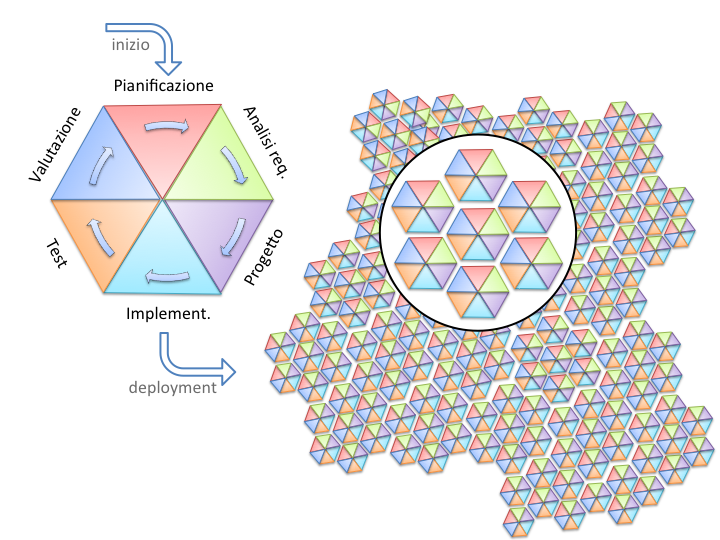
\includegraphics[scale=0.5]{img/modello_incrementale.png}
		\caption{Rappresentazione del modello incrementale\protect\footnotemark}
		\label{fig:modello_incrementale}
	\end{figure}

	\footnotetext{Fonte in \S\ref{rifinfo}}
	
    \include{sections/requisiti_sistema}
    \section{Configurazione}\label{configurazione}

Su richiesta di \II, tutti i servizi sono stati configurati sotto forma di container. È quindi possibile avviarli su macchine fisiche differenti, ma collegate in rete fra loro, con Docker.\\
Sempre sotto richiesta di \II viene utilizzato Rancher come software per la gestione dei container, quindi questa guida verterà principalmente sulla configurazione di \progetto utilizzando Rancher. %TODO riverere frase per ripetizione

\subsection{Requisiti di sistema}

	Non sono necessari particolari requisiti in modo da poter configurare e utilizzare il nostro prodotte, tuttavia valgono i requisiti minimi dei sistemi di terze parti che vengono utilizzati da \progetto.

	\subsubsection{Software}
		\begin{itemize}
			\item Docker\footnote{\url{https://docs.docker.com/v17.09/datacenter/ucp/2.1/guides/admin/install/system-requirements}}: è necessario avere installata e configurata correttamente almeno la versione v18.09.
			\item Docker Compose\footnote{\url{https://docs.docker.com/compose/install/}} :  nel caso si decidesse di utilizzare Docker Compose per l'avvio dei container è consigliata l'installazione e configurazione corretta della versione v3.7.
			\item Kubernetes\footnote{\url{https://kubernetes.io/docs/setup/independent/install-kubeadm}}: nel caso si decidesse di utilizzare Kubernetes per la gestione dei container è consigliata l'installazione e configurazione corretta della versione v1.13.
			\item Rancher\footnote{\url{https://rancher.com/docs/rancher/v2.x/en/installation/requirements/}}: nel caso si decidesse di utilizzare Rancher per la gestione grafica di oggetti Kubernetes contenenti i container Docker, è consigliata l'installazione e configurazione della versione v2.1.4.
			\item Kafka\footnote{\url{https://docs.confluent.io/current/installation/system-requirements.html}}: è necessario avere installata e configurata correttamente almeno la versione v2.12.
			\item GitLab\footnote{\url{https://git.ucd.ie/help/install/requirements.md}} 11.7
			\item Redmine\footnote{\url{https://www.easyredmine.com/faq/technical-info/176-hardware-and-software-requirements-for-server-solution}}: durante lo sviluppo di \progetto abbiamo utilizzato 4.0.1
		\end{itemize}
	
	%TODO rivedere
	GitLab e Redmine sono componenti esterne a \progetto, tuttavia vengono citate in quanto è possibile configurare tutto il progetto in un ambiente unico.\\
	Le versioni specificate possono essere trovate anche nella sezione ``Requisiti di vincolo'' del documento \AdRv.
	
	\subsubsection{Hardware}
	Per \progetto~non sono necessari ulteriori requisiti a livello hardware particolari se non quelli di cui hanno bisogno i software precedentemente elencati.

\subsection{Mappatura delle porte}
Per la configurazione di ciascun tipo servizio abbiamo deciso di dare un range di porte da poter esporre in modo tale da effettuare una separazione a logico.\\
Questa regola non influisce col corretto funzionamento di \progetto ma è solamente per non assegnare le porte in modalità casuale e facilitare le analisi di eventuali errori come anche la facile manutenzione e aggiunta di servizi.

La suddivisione delle porte è la seguente:

\begin{table}[H]
	\centering
	\begin{paddedtablex}[1.3]{\textwidth}{YYY}
		\thead{Servizio} & \thead{Porta inizio} & \thead{Porta fine}\\\toprule
		Software di terze parti& 30000& 30029\\\hline
		Kafka e servizi correlati& 30030& 30059\\\hline
		Producer& 30060& 30089\\\hline
		Consumer& 30090& 30119\\\hline
		Gestore personale& 30120& 30149\\
	\end{paddedtablex}
	\caption{Suddivisione delle porte}
\end{table}

La suddivisione che abbiamo utilizzato durante lo sviluppo ed alla consegna del progetto prevede la seguente esposizione delle porte:

\begin{table}[H]
	\centering
	\begin{paddedtablex}[1.3]{\textwidth}{YYY}
		\thead{Servizio} & \thead{Porta interna} & \thead{Porta esposta}\\\toprule
		Redmine& 3000& 30000\\\hline
		GitLab& 80& 30001\\\hline
		Kafka& 9092& 30030\\\hline
		Producer GitLab& 5000& 30060\\\hline
		Producer Redmine& 5000& 30061\\\hline
		Consumer Telegram& 30090& \\\hline
		Consumer Email& 30091& \\\hline
		Producer Gestore personale& 30120& 5000\\\hline
		Consumer Gestore personale& 30121& \\
	\end{paddedtablex}
	\caption{Configurazione delle porte in fase di sviluppo e consegna}
\end{table}

Le specifiche relative alla configurazione delle porte in Rancher possono essere trovate nella pagina dedicata\footnote{\url{https://rancher.com/docs/rancher/v2.x/en/installation/references/}} sulla sezione della documentazione presente nel loro sito.

\subsection{Configurazione servizi principali container}

	\subsection{Webhook}
	Per il corretto invio dei webhook (in formato JSON) da parte dei software che comunicano con i nostri Producer è necessaria una piccola configurazione:
	
	\paragraph{Redmine}
	
		\subparagraph{Configurazione del plugin}
	
		scaricarlo nella cartella... 
		verificare in sezione admin in configurazioni parte amministratore...
	
	L'implementazione per Redmine si appoggia sul plugin \texttt{redmine\_webhook}, raggiungibile al link
	\url{https://github.com/suer/redmine_webhook}.
	
	Questo plugin implementa il concetto di Hook offerto dalla API di Redmine, inviando a un determinato URL
	un \gloss{payload} costituito da un file JSON quando un evento si innesca, contenente le informazioni relative
	a tale evento.
	
	Per installarlo su un'istanza di Redmine, seguire le istruzione riportate nel README presente nella repository.
	
		\subparagraph{Configurazione destinazione}
		Per aggiungere una destinazione del webhook per un progetto, andare nella sezione relativa al webhook all'interno del menu del progetto...
		...aggiungere la destinazione e premere add..
		%todo inserire immagine
	
		\subparagraph{Eventi supportati}
		\begin{itemize}
			\item Comments
		\end{itemize}
	
		
	\paragraph{GitLab}
		\subparagraph{Configurazione webhook nella rete locale}
		È necessario abilitare l'invio dei webhook a dispositivi presenti nella stessa rete dalla parte amministrativa.
		Questo può essere effettuato accedendo con un account con privilegi amministratore all'indirizzo:
		\begin{center}
			\texttt{\url{/admin/application_settings/network}}
		\end{center}
		Per abilitare questa funzionalità cliccare sul riquadro rappresentato nell'immagine e che si trova all'indirizzo sopra indicato.
		\begin{figure}[H]
			\centering
			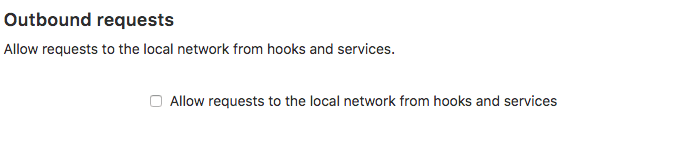
\includegraphics[width=13cm]{img/webhook_gitlab_setup.png}\\
			\caption[Webhook, GitLab]{Configurazione webhook con destinazione in rete locale}
		\end{figure}
		Ulteriori informazioni al riguardo possono essere trovate nella pagina\footnote{\url{https://docs.gitlab.com/ee/security/webhooks.html}} relativa a questo argomento sulla parte del sito relativa alla documentazione di GitLab.
		\subparagraph{Configurazione destinazione}
		Successivamente si può aggiungere indirizzo di destinazione un webhook al progetto andando sulle impostazioni:
		\begin{center}
			\texttt{Settings > Integrations}
		\end{center}
		Da qui si possono selezionare gli eventi di interessi per i quali i webhook verranno attivati (attenzione: \progetto~non supporta tutti gli eventi, solamente quelli richiesti da \II).
		Nel campo relativo all'URL di destinazione inserire l'indirizzo, con relativa porta (nel nostro caso quella specificata nella Tabella 2), su cui il Producer GitLab è in ascolto.
		\subparagraph{Eventi supportati}
		Per GitLab gli eventi supportati sono:
		\begin{itemize}
			\item Push events
			\item Comments
			\item Issues events
		\end{itemize}


---


	%TODO RIVEDERE
	La configurazione dei consumer e dei producer sono composte da file json contenti informazioni come ad esempio la mail di invio e la password relativa utilizzate per accedere al server mail.
	Queste possono essere modificate in modo tale da rispecchiare la configurazione che si vuole usare.
	
\subsection{Servizi aggiuntivi}
Aggiungere servizio necessario per il monitoraggio di kafka
Altri servizi per monitoraggio ?
    %\newpage
\section{Tecnologie e scelte relative al progetto}
	L'obiettivo di questo paragrafo è descrivere in maniera specifica come \progetto\ andrà a interfacciarsi con le tecnologie.\\
	Per ciascuna di queste è previsto un \gloss{microservizio}, il quale avrà come scopo quello di fare da tramite tra lo strumento che genera il messaggio e quello che lo riceve.\\
	Questo pattern si chiama \gloss{Publisher / Subscriber} e utilizza uno strumento intermedio detto Broker per lo smistamento dei messaggi e la gestione dei flussi.

	\begin{figure}[H]
		\centering
		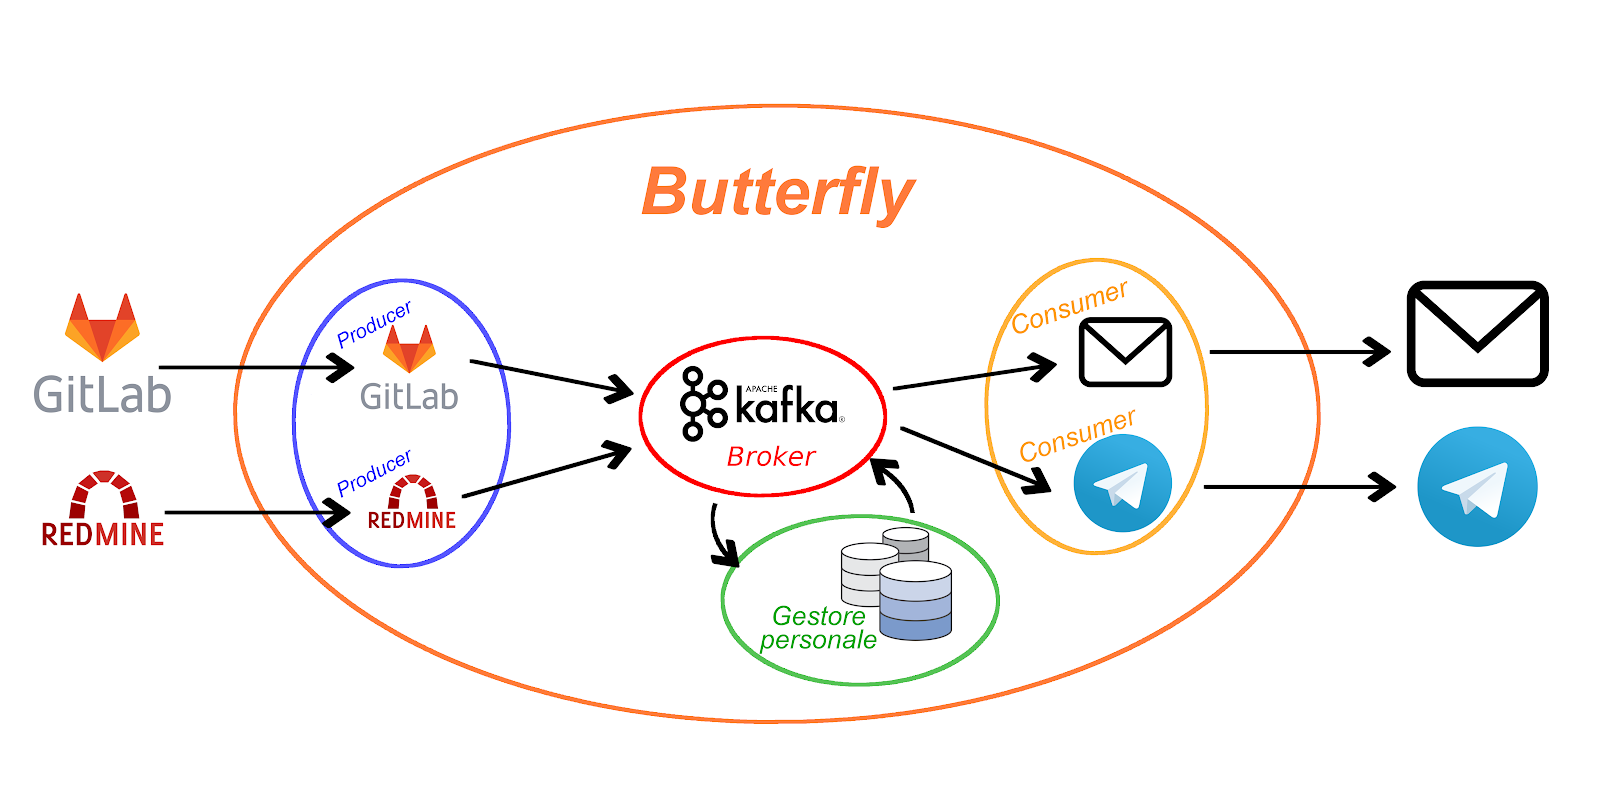
\includegraphics[width=\textwidth]{img/butterfly.png}\\
		\caption{Visione generale del sistema \progetto}
		\label{fig:butterfly}
	\end{figure}
	L'immagine precedente rappresenta una suddivisione del sistema in quattro sezioni principali:
	\begin{itemize}
		\item \progetto\ (arancione)
		\item Producer (azzurro)
		\item Broker (rosso)
		\item Consumer (verde)
	\end{itemize}
	Questa scomposizione permette di analizzare più approfonditamente i vari sottosistemi del prodotto in rapporto alle tecnologie esterne a Butterfly (GitLab, Redmine, Telegram ed e-mail), ai microservizi interni come i Producer / Consumer associati e il Broker.
	
	\subsection{Producer}
	
		Per ciascuno degli strumenti che invia messaggi verso il sistema è necessario creare una componente applicativa di tipo Producer che li riceva e li elabori inoltrandoli successivamente verso il Broker.
		Le tecnologie dalle quali vengono ricevuti i messaggi sono elencate di seguito in ordine di priorità in base a quanto richiesto dal \gloss{committente}.
		\begin{itemize}
			\item Redmine
			\item GitLab
			\item SonarQube
		\end{itemize}
		\gruppo\ ha scelto di sviluppare i Producer per le prime due applicazioni in base alle priorità suggerite da \II\ nel capitolato, lasciando l'applicativo relativo a SonarQube come opzionale.
		
		Ciascun messaggio ricevuto da queste tecnologie verrà analizzato dal Producer associato che ne ricercherà al suo interno keyword che ne indicano il Topic.
		Queste sono preimpostate da una persona incaricata dall'azienda che le inserisce nel database.
		
		\subsubsection{Redmine}
		Ciascuna istanza di Redmine permette l'utilizzo di webhook\footnote{Riferirsi alla voce ``Webhook di Redmine'' alla sezione \S\ref{sec:RiferimentiInformativi}} che inviano segnalazioni al Producer alla modifica del progetto.
		Queste vengono ricevute dal server tramite un microservizio che resta in ascolto, aggiornando in base a quello che riceve i dati presenti sul gestore personale e inoltrando le notifiche ai Consumer interessati.
		In particolare, le modifiche relative al progetto prese in considerazione sono:
		\begin{itemize}
			\item Apertura issue
		\end{itemize} 
		
		\subsubsection{GitLab}
		Ciascuna istanza di GitLab, online o in un server locale interno dell'azienda, mette a disposizione la configurazione di webhook\footnote{Riferirsi alla voce ``Webhook di GitLab'' alla sezione \S\ref{sec:RiferimentiInformativi}} che, alla modifica della \gloss{repository}, manda un messaggio con le informazioni dei cambiamenti, inseriti nella repository, a un microservizio capace di aggiornare i dati presenti nel gestore personale e, come per Redmine, inoltrare le notifiche ai Consumer interessati.
		In particolare, le modifiche relative alla repository prese in considerazione sono:
		\begin{itemize}
			\item Commit
			\item Apertura \gloss{issue}
			\item Chiusura issue
		\end{itemize}
		Le segnalazioni sono generate da commit contenenti \gloss{keyword} preimpostate.
		
%		\subsubsection{SonarQube}
%		Come GitLab, anche SonarQube prevede l'utilizzo di Webhooks\footnote{\url{https://docs.sonarqube.org/latest/project-administration/Webhooks/}} che dopo ciascuna build comunica il risultato e le informazioni relative ad essa ad un microservizio capace di aggiornare i dati presenti nel gestore personale e, anche in questo caso, inoltrare le notifiche ai customer interessati.
		
	\subsection{Broker}
	
		Il ruolo del Broker è quello smistare i messaggi in base ai Topic con cui questi sono contrassegnati verso i vari microservizi con cui l'utente ha deciso che gli venga inoltrata la notifica.
		L'azienda consiglia di utilizzare come Broker per i messaggi \gloss{Apache Kafka}.
	
		\subsubsection{Apache Kafka}
		\gloss{Apache Kafka} è un software \gloss{open source} che permette la lettura e la scrittura di messaggi su stream di dati.
		Questi messaggi arrivano dai microservizi Producer che ricevono le notifiche di applicazioni di terze parti e mandandole verso il Broker. Questo le elabora analizzandone il contenuto e contrassegnandole con Topic che verranno utilizzati per l'inoltro ai Consumer e successivamente agli utenti finali, i quali possono abbonarsi a più Topic e gestendo le proprie preferenze.		
	
	\subsection{Consumer}
		Come per gli strumenti precedentemente elencati, anche per quelli su cui il messaggio andrà ad essere inoltrato, è necessaria la creazione di un microservizio in grado di fare da tramite tra Broker e \gloss{client} dello strumento.
		Le tecnologie alle quali vengono inoltrati i messaggi sono elencate di seguito in ordine di priorità in base a quanto richiesto dal committente.
			
		\subsubsection{Telegram}
		Telegram permette l'interazione in maniera automatica con gli utenti tramite \gloss{bot} che possono essere configurati per mandare messaggi ricevuti da strumenti di terze parti.
		Il Broker manda i messaggi ad un microservizio che si occupa della trasmissione effettiva al bot di Telegram.
		%https://core.telegram.org/bots
		
		\subsubsection{E-mail}
		Per inoltrare le e-mail agli utenti finali è necessario un microservizio che sfrutta un server di posta in modo tale da poter ricevere i messaggi dal Broker e poi mandarli all'indirizzo specificato.
		%https://realpython.com/python-send-email/
		
%		\subsubsection{Slack}
%		È possibile utilizzare le API di Slack per poter mandare push notifications ai canali o alle persone interessate specificando il nome del canale (o lo username della persona), testo del messaggio, e lo username che verrà mostrato per il mittente.
%		%https://www.confluent.io/blog/real-time-syslog-processing-with-apache-kafka-and-ksql-part-2-event-driven-alerting-with-slack/
	
	\subsection{Gestore personale}
	Il gestore personale è quel \gloss{componente} che permette agli utenti di impostare le proprie preferenze per il canale di inoltro dei messaggi ed i Topic a cui ci si iscrive, interfacciandosi dunque con l'intero sistema.
	È previsto come un'applicazione web installata in un server interno all'azienda accessibile dai dipendenti interessati, i quali potranno quindi modificare, perciò con la possibilità di aggiungere e rimuovere, impostazioni come Topic a cui si è iscritti e modalità di ricezione dei messaggi.
	
	\subsection{Container Software}
	
		Un container software simula questo ambiente virtuale dove è possibile testare e mantenere le proprie applicazioni, permettendo di aumentare l'efficienza riducendone i costi e simulando l'esecuzione di sistema operativo su una macchina con \gloss{risorse} condivise.
		
		\subsection{Differenza tra container e macchina virtuale}
		A differenza delle \gloss{macchine virtuali}, dove lo stato dell'ambiente viene salvato su disco occupando memoria, i container si adattano in maniera più performante all'applicativo richiesto, in quanto il loro scopo è quello di massimizzare la quantità delle applicazioni in esecuzione riducendo al minimo il numero delle macchine per eseguirla.
		Sono quindi più leggeri, occupando meno memoria su disco e impiegando meno risorse. Purtroppo al termine della loro esecuzione non viene salvato lo stato, a meno che non sia esplicitamente richiesto.
		
		\subsubsection{Docker e Dockerfile}
		L'azienda consiglia di utilizzare \gloss{Docker} per la semplicità e perché si adatta all'architettura a microservizi.
		La configurazione avverrà tramite un \gloss{dockerfile} in cui verranno specificate informazioni come sistema operativo, script di avvio, numero di istanze ed altri parametri specifici.

	\subsection{Utenti}
		\subsubsection{Amministratore}
		\subsubsection{Utente finale}
		
	\subsection{Topic}
    \section{Architettura}\label{Architettura}

In questa sezione descriviamo brevemente l'architettura del sistema \progetto.

L'architettura adottata è \gloss{event-driven}: ogni componente è isolato e asincrono,
e comunica attraverso interfacce scambiandosi messaggi tramite il broker Apache Kafka.

Il sistema si divide principalmente in tre insiemi di componenti:

\begin{itemize}
    \item Producers
    \item Gestore Personale
    \item Consumers
\end{itemize}

\subsection{Producers}
Il Producer è il componente che resta in ascolto degli webhook provenienti dal suo applicativo specifico (e.g. Redmine, GitLab).
Ha lo scopo di immettere i messaggi su Kafka in formato \gloss{JSON}, conservando solo i campi di interesse e aggiungendone eventualmente di propri.

Al momento della stesura di questo manuale, i Producer implementati sono due:
\begin{itemize}
    \item RedmineProducer
    \item GitlabProducer
\end{itemize}

L'algoritmo di invio dei messaggi differirà solamente nella modalità in cui verrà formato il messaggio finale: per questo motivo abbiamo deciso di utilizzare
il design pattern \gloss{Template Method} per l'implementazione dell'algoritmo. Le classi concrete avranno esclusivamente il compito di implementare
il parser degli webhook e il metodo del Producer \texttt{webhook\_kind()}.


\subsubsection{RedmineProducer}

Il Producer di Redmine si occupa di ascoltare gli webhook provenienti dai progetti di Redmine che hanno configurato la porta relativa al componente,
e di immettere nella coda \textit{redmine} di Kafka i messaggi.

Nel seguente diagramma di sequenza è possibile vedere il flusso di esecuzione, che parte dall'arrivo di un webhook da Redmine e si conclude con
l'inoltro del messaggio sulla coda \textit{redmine} di Kafka.

\begin{figure}[H]
    \centering
    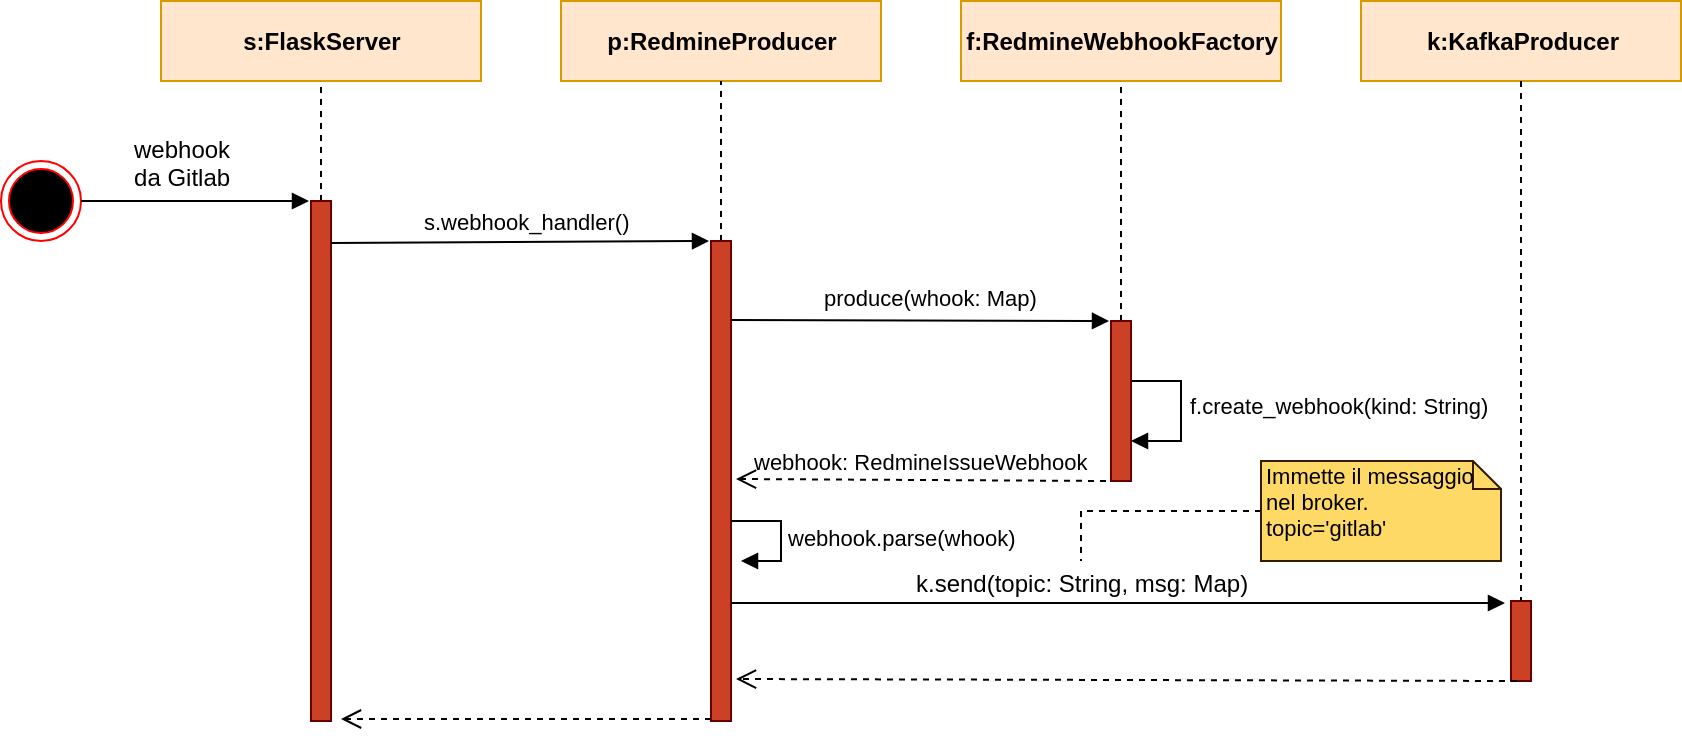
\includegraphics[width=\textwidth]{img/Producer-MsgRedmine.png}\\
    \caption[Diagramma di sequenza di RedmineProducer]{Diagramma di sequenza per la ricezione di un messaggio su RedmineProducer e invio del messaggio su Kafka}
    % \label{fig:producers}
\end{figure}

\paragraph{Diagramma dei package}

Il package \texttt{producer} ha tre dipendenze esterne:
\begin{itemize}
    \item \texttt{Flask}, classe concreta del package di libreria \texttt{flask}: è il server che si mette in ascolto degli webhook provenienti da Redmine.
    \item \texttt{KafkaProducer}, classe concreta del package di libreria \texttt{kafka-python}: ha il compito di interfacciarsi con il broker Kafka e di immettere
        in esso i messaggi. È costruito su di esso un \gloss{Adapter}, in cui KafkaProducer viene adattato all'astrazione \texttt{Producer}.
    \item Package \texttt{webhook}: ha il compito di effettuare il parsing dei messaggi in entrata.
\end{itemize}

\begin{figure}[H]
    \centering
    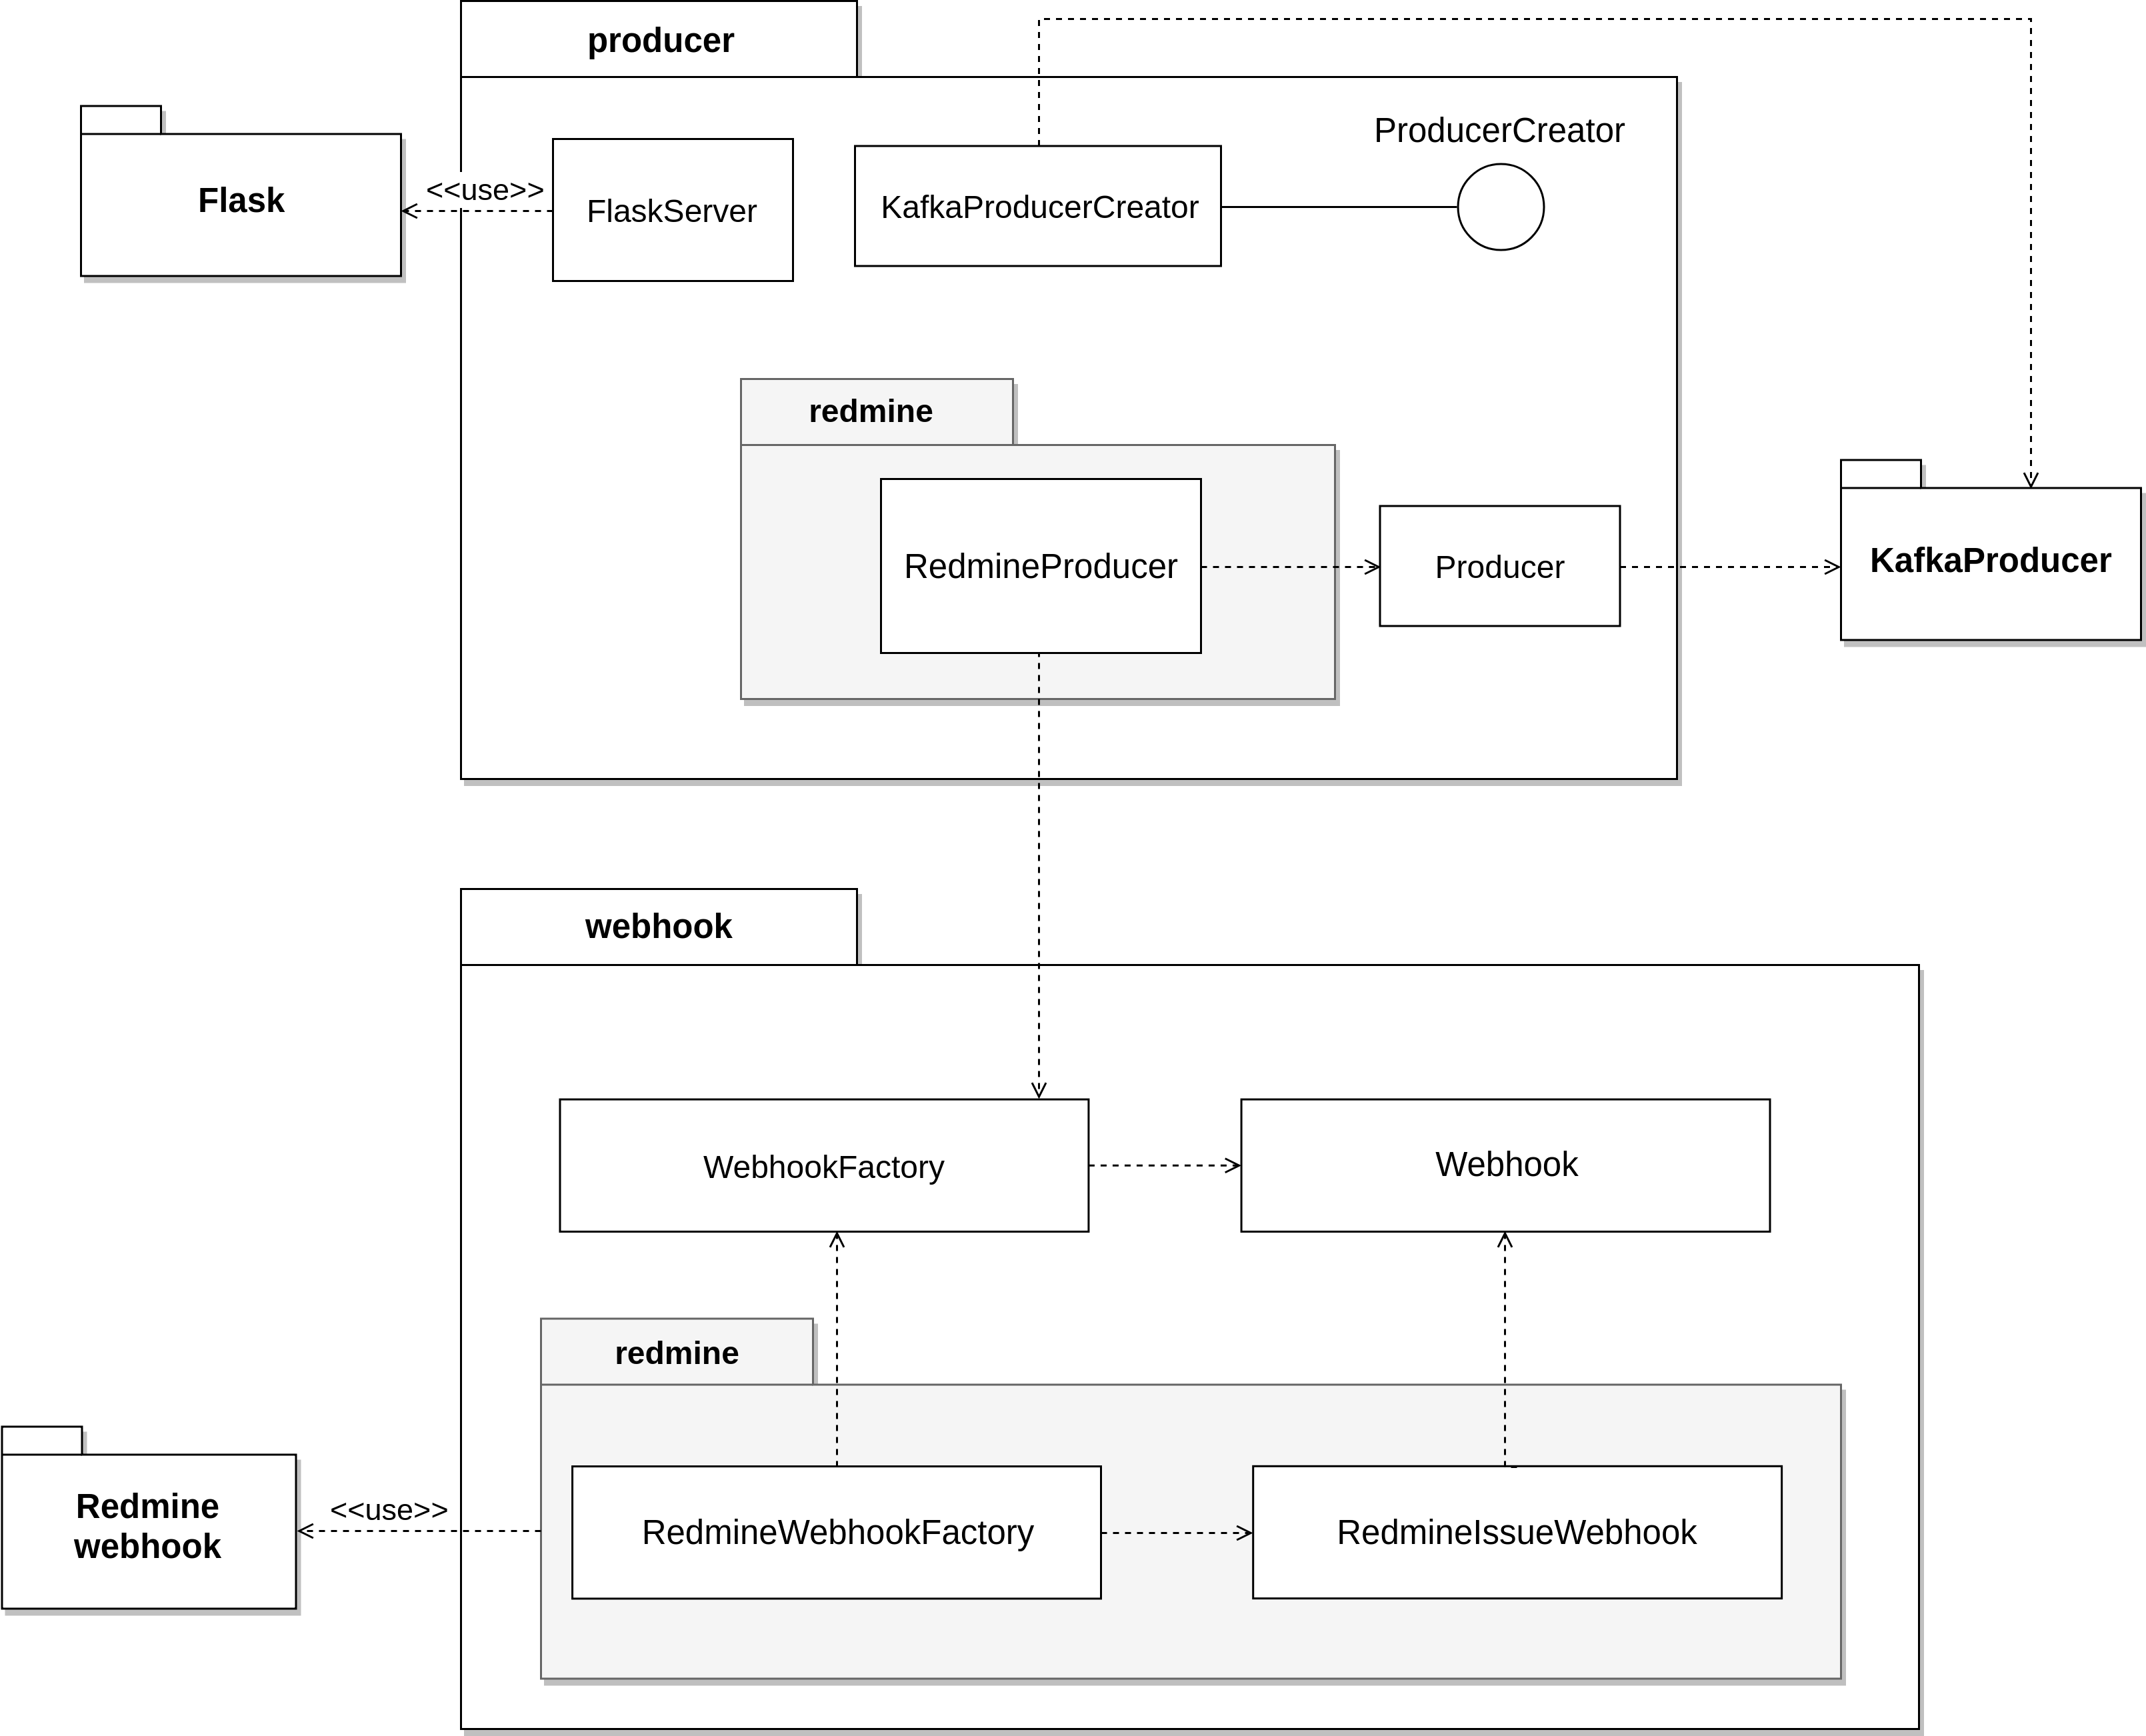
\includegraphics[width=\textwidth]{img/Package-RedmineProducer.png}\\
    \caption{Diagramma dei package di RedmineProducer}
    \label{fig:producers}
\end{figure}

\paragraph{Diagramma delle classi}

\begin{figure}[H]
    \centering
    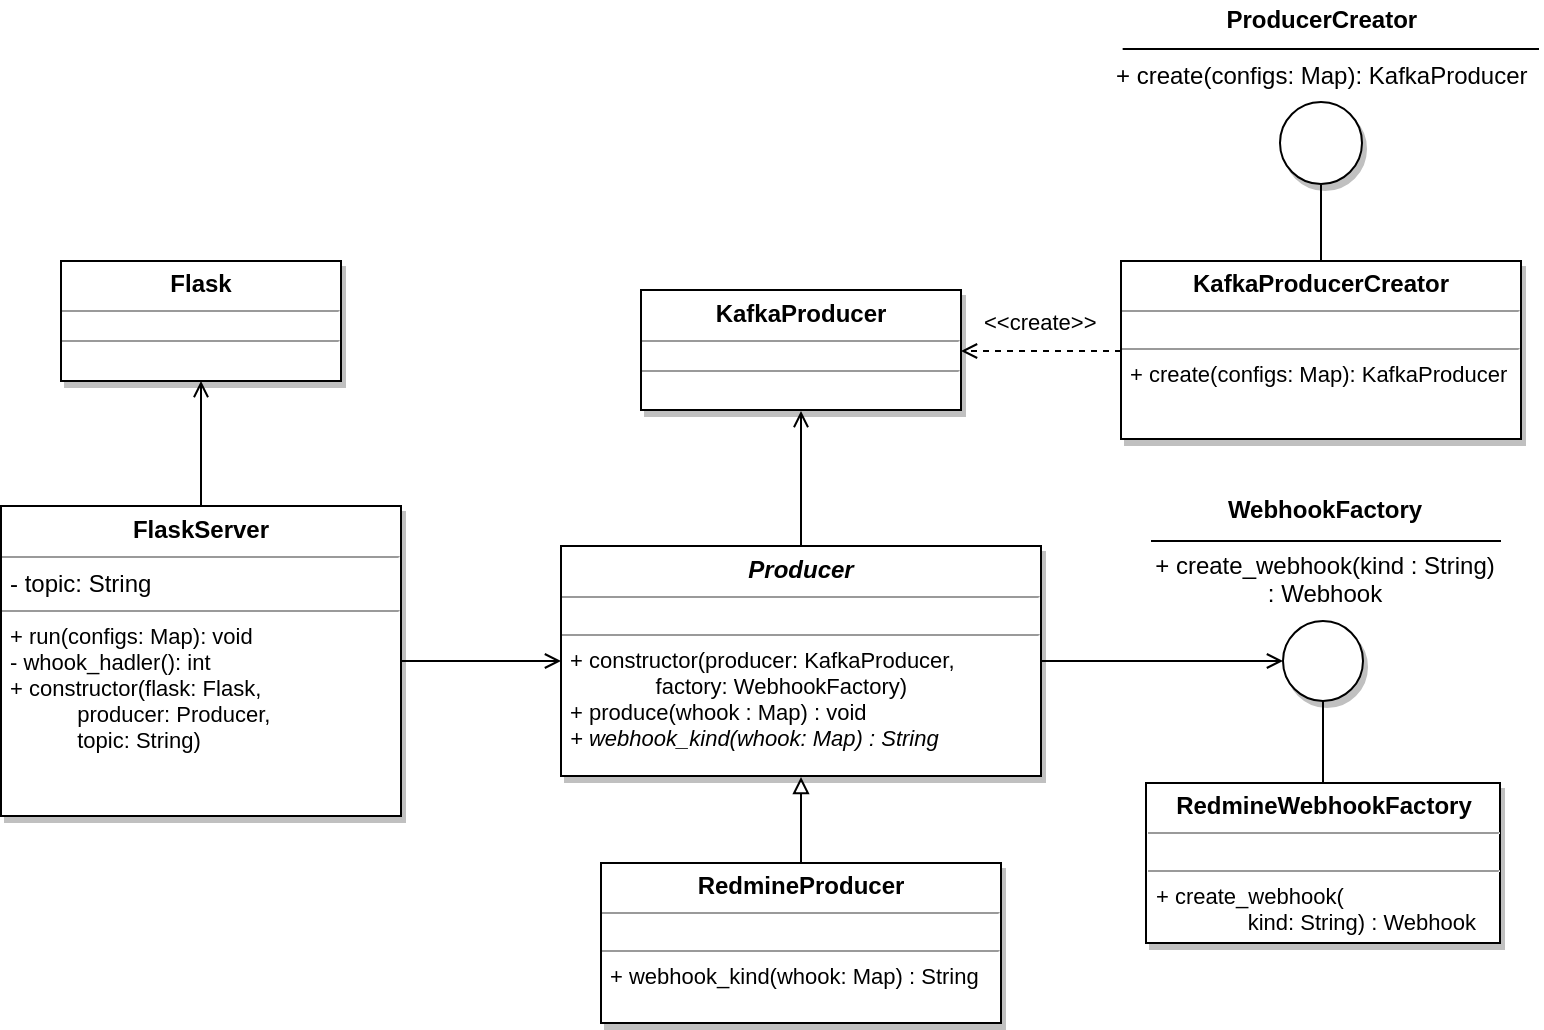
\includegraphics[width=\textwidth]{img/Producers-RedmineProducer.png}\\
    \caption{Diagramma delle classi di RedmineProducer}
    % \label{fig:producers}
\end{figure}

Per fare il parsing dei webhook, \texttt{RedmineProducer} si appoggia alla gerarchia \texttt{Webhook}.
Ogni istanza di \texttt{RedmineProducer} ha un riferimento a una \texttt{WebhookFactory}: quando viene
catturato un webhook da Redmine, chiama il metodo \texttt{create\_webhook(kind)} della
factory associata, passandogli come parametro la tipologia di webhook, in formato stringa.

Essa si occuperà di creare il parser di webhook adeguato al messaggio in entrata.
La classe concreta derivata da \texttt{Webhook} costruisce il messaggio con i campi di interesse da
immettere nella coda di Kafka, e lo restituisce al Producer.

Per Redmine, è presente una sola tipologia di webhook. Tenendo a mente l'\gloss{open-closed principle},
è stata implementata la gerarchia relativa ai webhook per permettere agli sviluppatori di poterne facilmente
aggiungere di nuovi.

\begin{figure}[H]
    \centering
    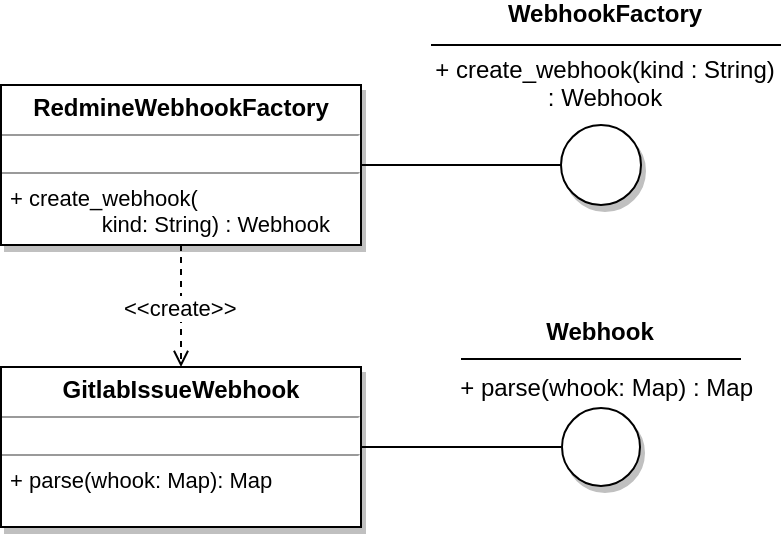
\includegraphics[width=0.6\textwidth]{img/Producers-RedmineWebhook.png}\\
    \caption{Diagramma delle classi di RedmineWebhookFactory}
    % \label{fig:producers}
\end{figure}



\subsubsection{GitlabProducer}
Il Producer di GitLab si occupa di ascoltare gli webhook provenienti dai progetti di GitLab
che hanno configurato la porta relativa al componente, e di immettere nella coda gitlab di
Kafka i messaggi.

Esso è implementato allo stesso modo di quello di Redmine, per cui non verrà ripetuta l'analisi delle
funzionalità che sono identiche al Producer di Redmine.

Per tenere isolate
le componenti, i diagrammi sono stati totalmente separati, anche se le classi risiedono nello stesso package.
Sarà compito dei Dockerfile copiare solamente i file necessari al componente specifico per poter mantenere
isolato il container.


\paragraph{Diagramma dei package}

\begin{figure}[H]
    \centering
    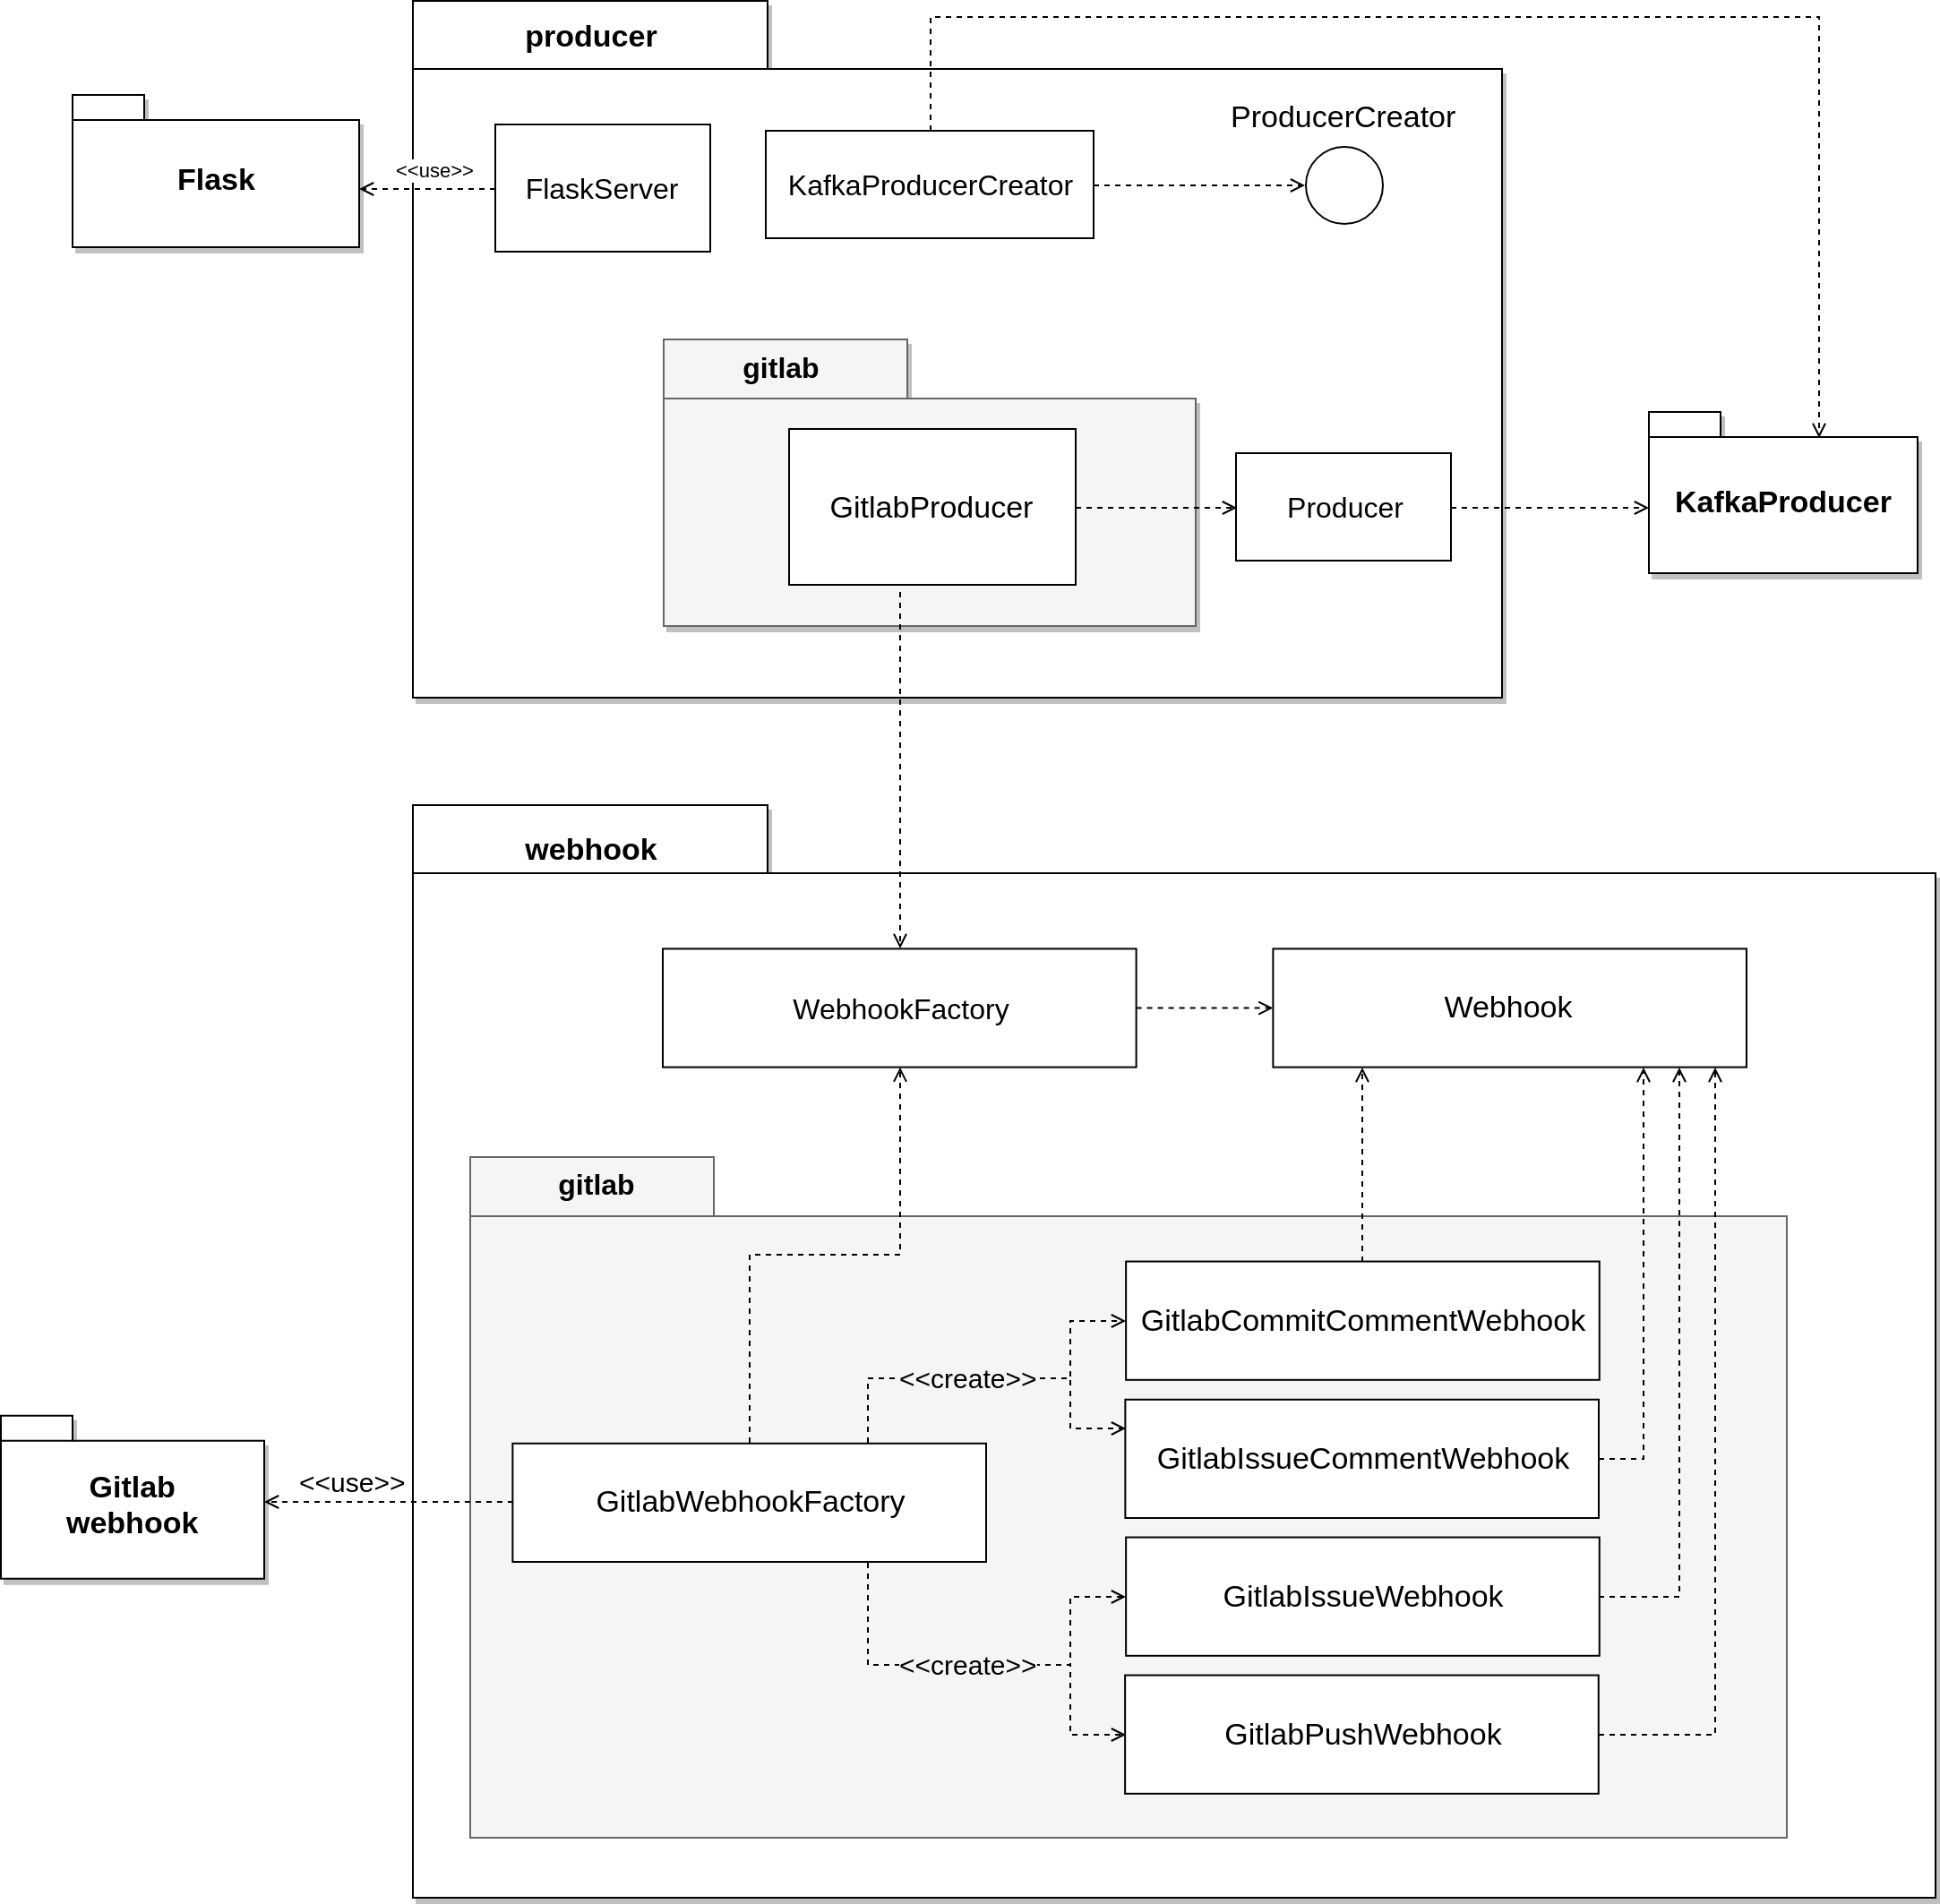
\includegraphics[width=\textwidth]{img/Package-GitLabProducer.png}\\
    \caption{Diagramma dei package di GitlabProducer}
    \label{fig:webhook}
\end{figure}


\paragraph{Diagramma delle classi}

\begin{figure}[H]
    \centering
    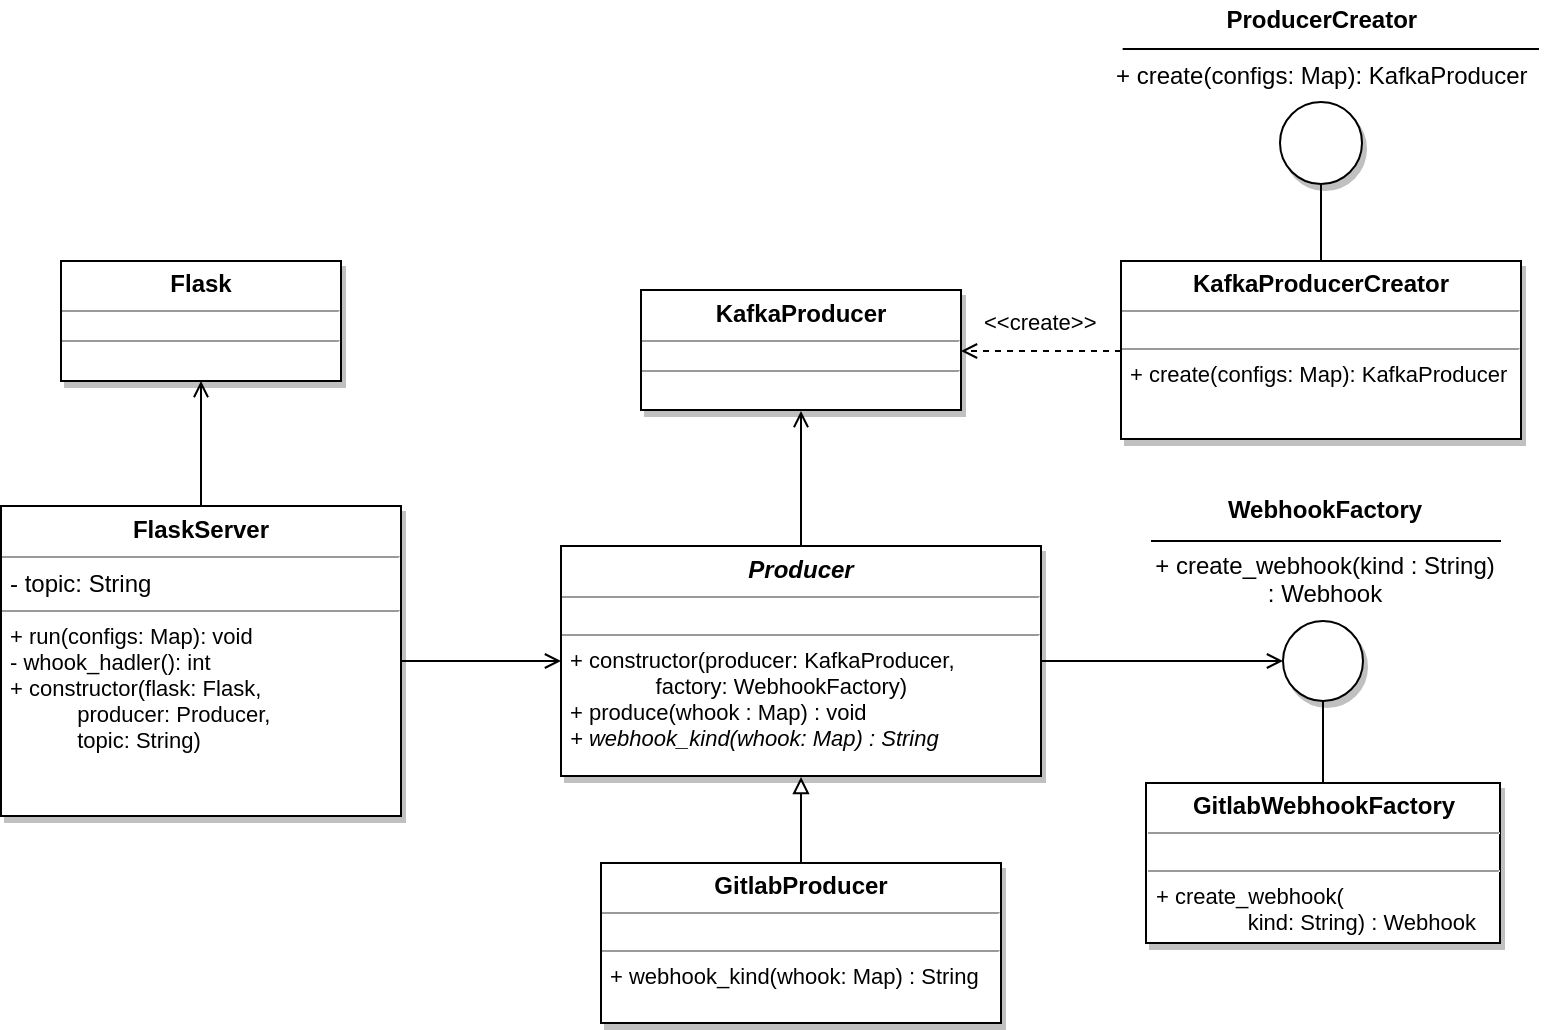
\includegraphics[width=\textwidth]{img/Producers-GitlabProducer.png}\\
    \caption{Diagramma delle classi di GitlabProducer}
    % \label{fig:producers}
\end{figure}

Abbiamo implementato per \texttt{GitlabProducer} 4 tipologie di \texttt{Webhook}.
Il parametro \texttt{kind} del metodo \texttt{create\_webhook(kind)} può quindi assumere 4 valori, in base al quale
\texttt{GitlabWebhookFactory} costruirà un parser di \texttt{Webhook} apposito:
\begin{itemize}
    \item '\texttt{issue}': verrà istanziato un \texttt{GitlabIssueWebhook}.
    \item '\texttt{push}': verrà istanziato un \texttt{GitlabPushWebhook}.
    \item '\texttt{issue-comment}': verrà istanziato un \texttt{GitlabIssueCommentWebhook}.
    \item '\texttt{commit-comment}': verrà istanziato un \texttt{GitlabCommitCommentWebhook}.
\end{itemize}

Questo è un pattern creazionale specifico: \gloss{Factory Method}.


\begin{figure}[H]
    \centering
    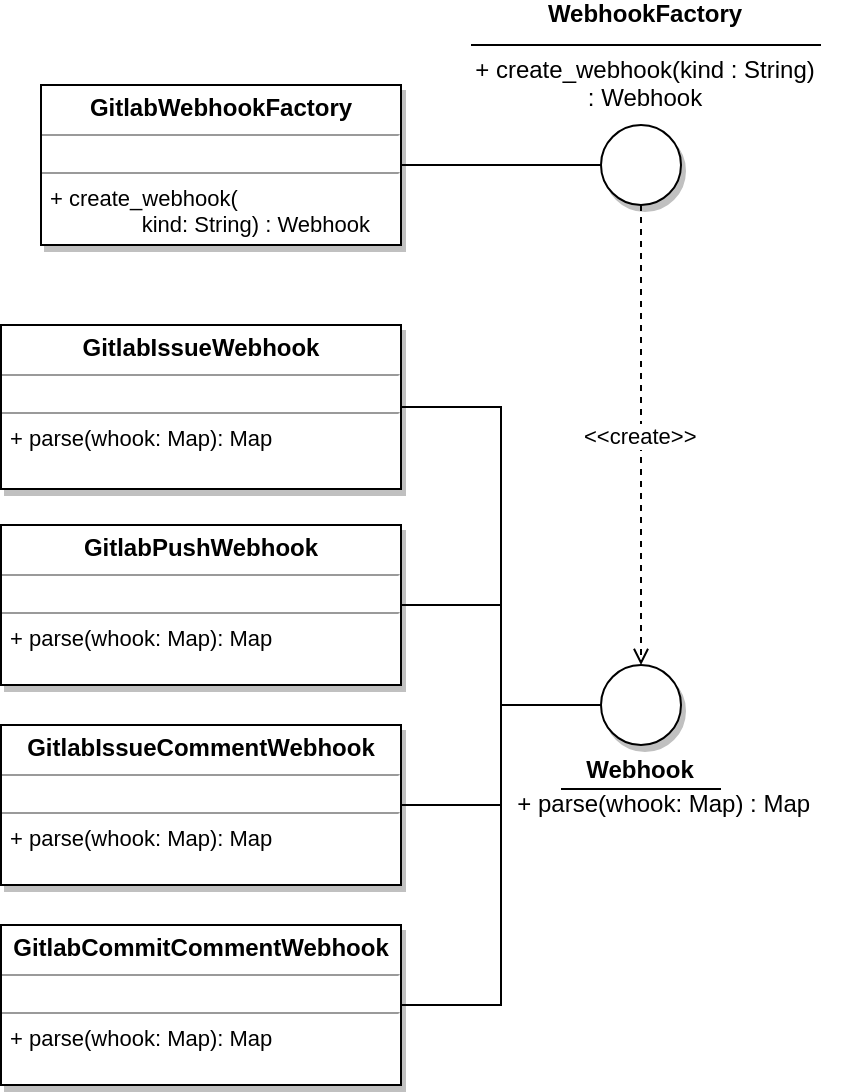
\includegraphics[width=0.6\textwidth]{img/Producers-GitlabWebhook.png}\\
    \caption{Diagramma delle classi di GitlabWebhookFactory}
    % \label{fig:producers}
\end{figure}



\subsection{Gestore Personale}

\subsubsection{Diagramma dei package}
Il Gestore Personale è la componente con la logica più complessa del sistema Butterfly. Esso ha un proprio KafkaProducer e KafkaConsumer
che si occupano rispettivamente di ricevere i messaggi da Kafka e reinserirli nelle code relative ai Consumer finali. Per stabilire il destinatario e il Consumer finale appropriato, il Client del Gestore Personale interroga MongoDB per ottenere le informazioni relative ad i giorni di indisponibilità, la priorità dei progetti e la piattaforma di messaggistica sul quale ricevere la notifica per ogni utente.
Tutte queste informazioni vengono inserite in MongoDB attraverso la View. \par
Questa prima parte riguarda la sezione del gestore personale che va a interfacciarsi con l’utente adottando un’architettura MVC pull model, ovvero \texttt{rest\_hadler} nella figura \ref{GP-Package}.
L’unica cosa che fa le View è inoltrare i comandi ricevuti dall’utente all’\gloss{API REST}. \par
Esiste poi invece anche un'altra parte chiamata \texttt{message\_processor} che è collegata al MongoDB.
Questo perchè deve poter analizzare i dati dei vari utenti in modo da capire dove inserire su Kafka il mesaggio elaborato.

\begin{figure}[H]
    \centering
    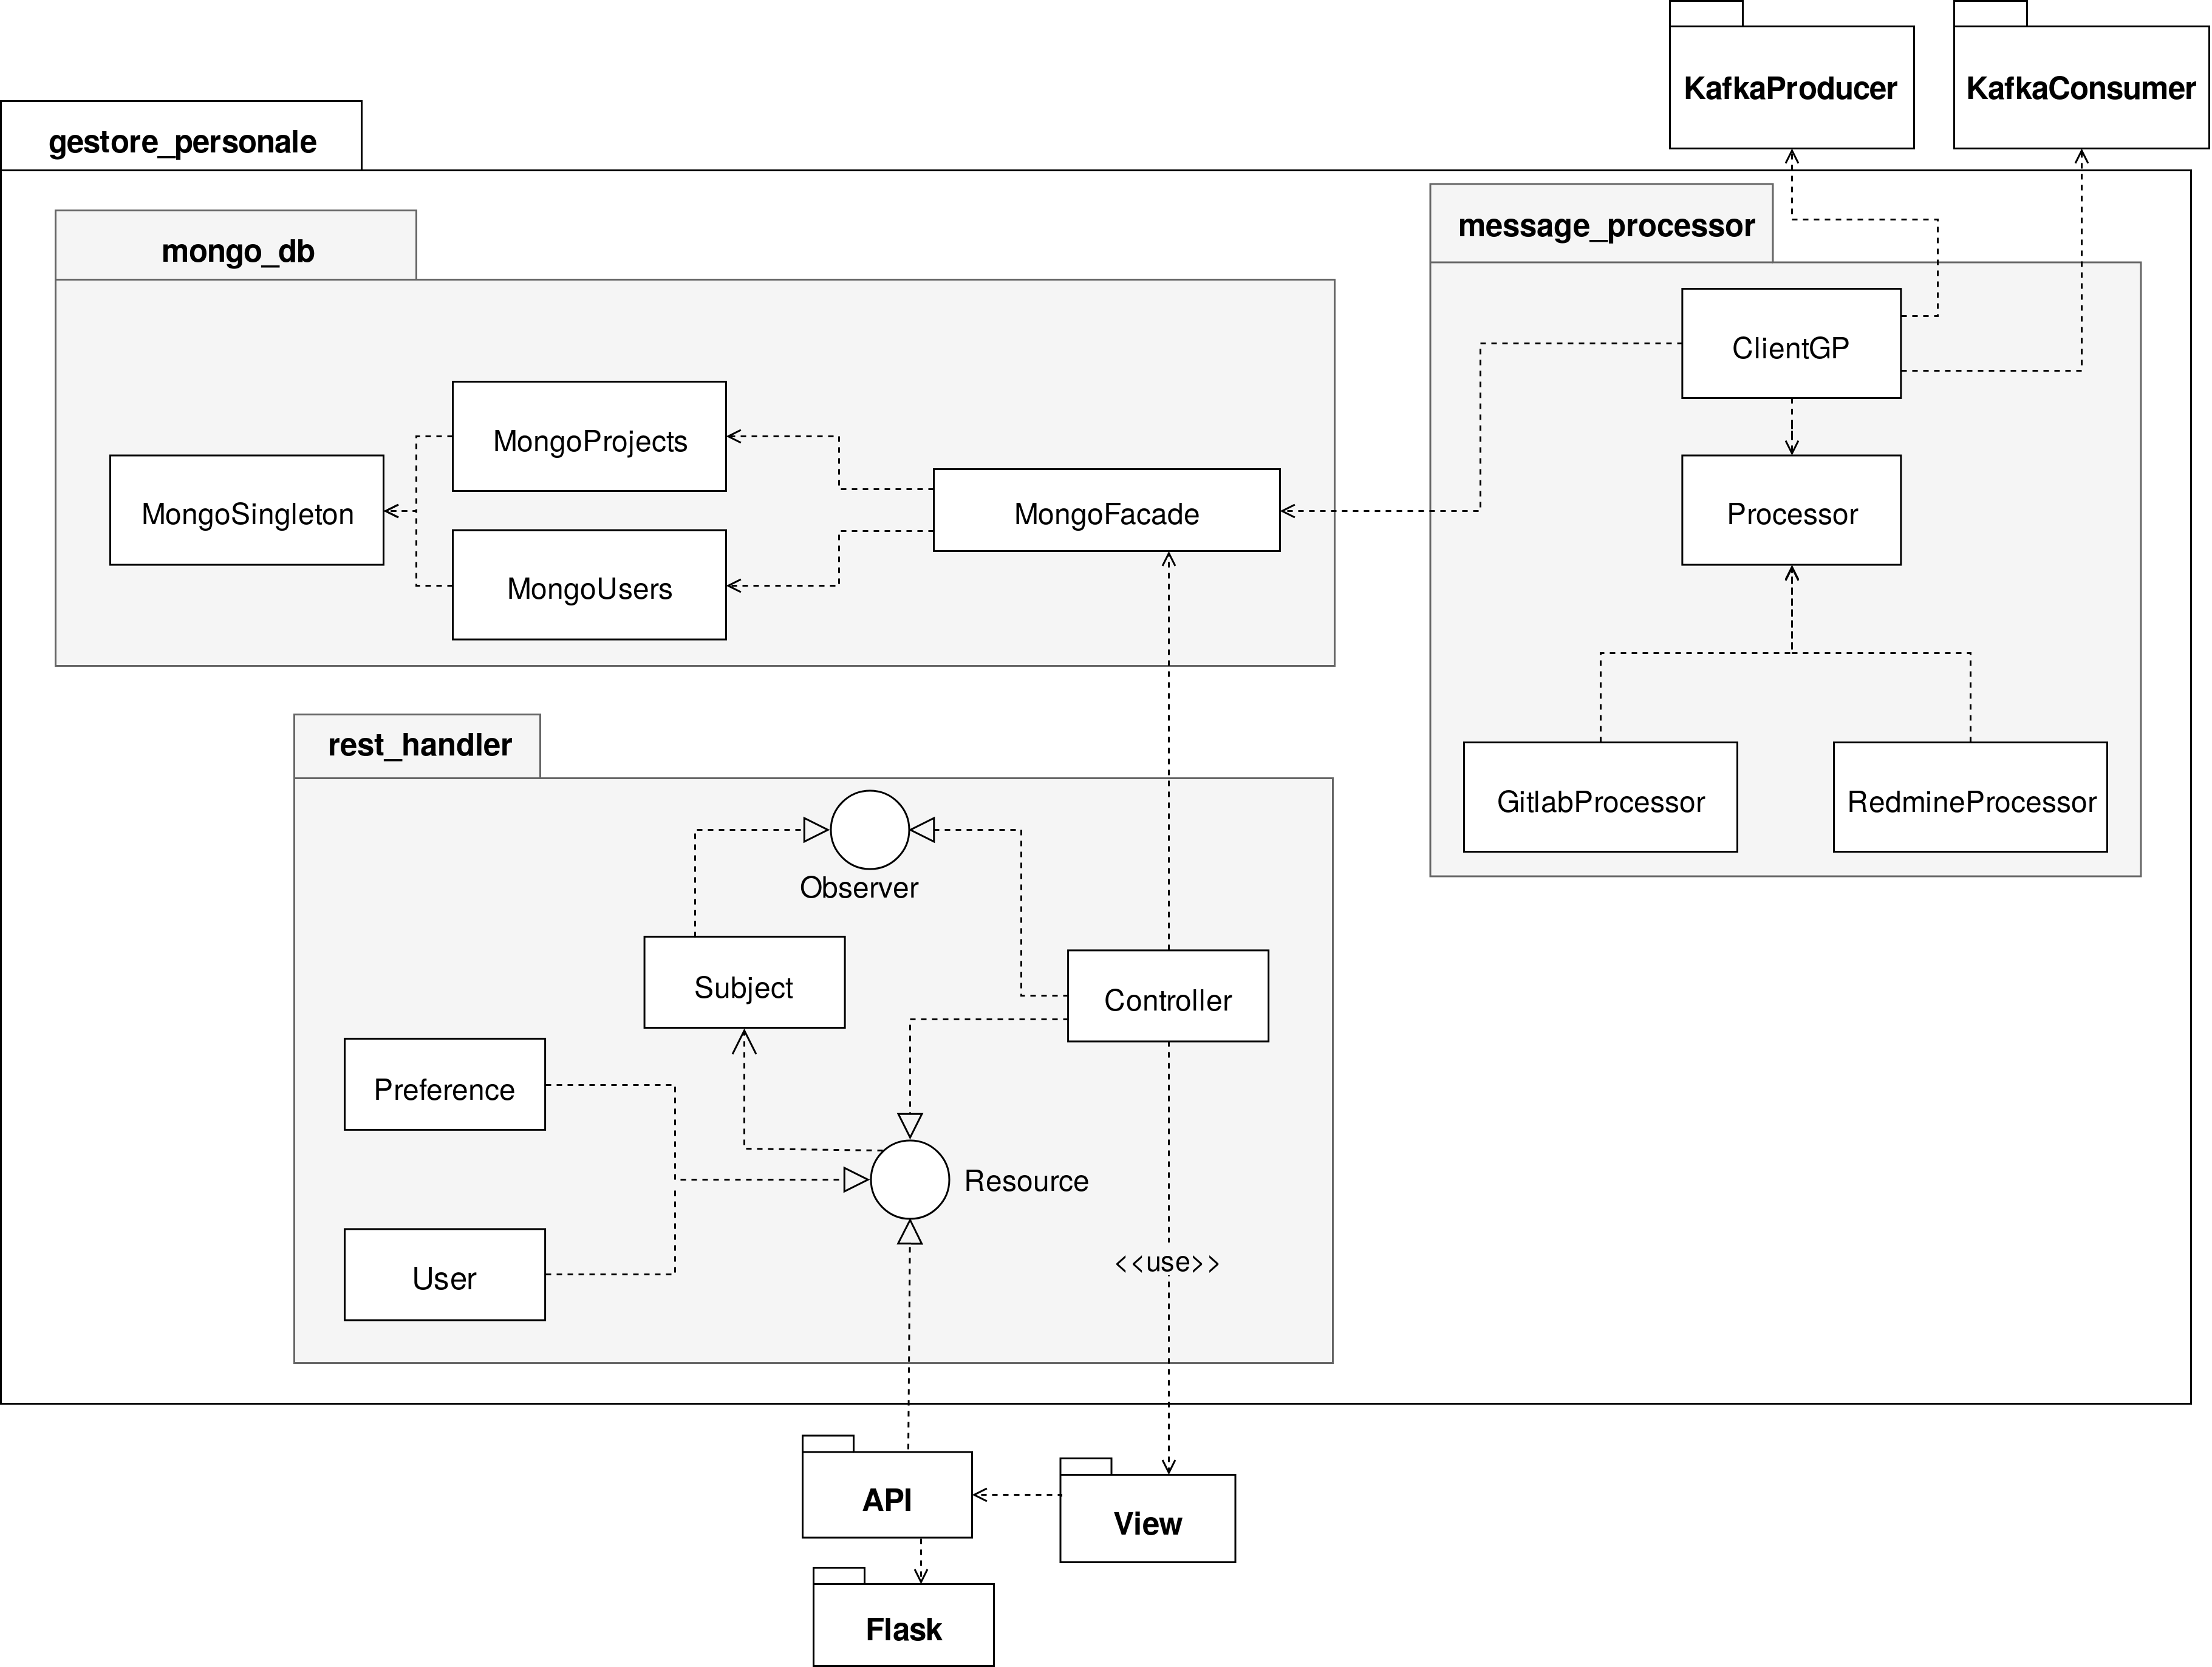
\includegraphics[width=\textwidth]{img/Package-GestorePersonale.png}\\
    \caption{Diagramma dei package del Gestore Personale}
    \label{GP-Package}
\end{figure}

\subsubsection{Mongo} \label{Mongo}
\gloss{MongoDB} è un database non relazionale orientato all'utilizzo di documenti, e non di tabelle come nei database relazionali. Ci è molto utile in questo progetto perché ci dà la possibilità di aggiungere dati ai documenti senza modificarne la struttura.
Questo lo rende un database molto estensibile, quindi uno sviluppatore può facilmente ampliare le informazioni in esso contenute.

    \paragraph{Diagramma delle classi}

    \begin{figure}[H]
        \centering
        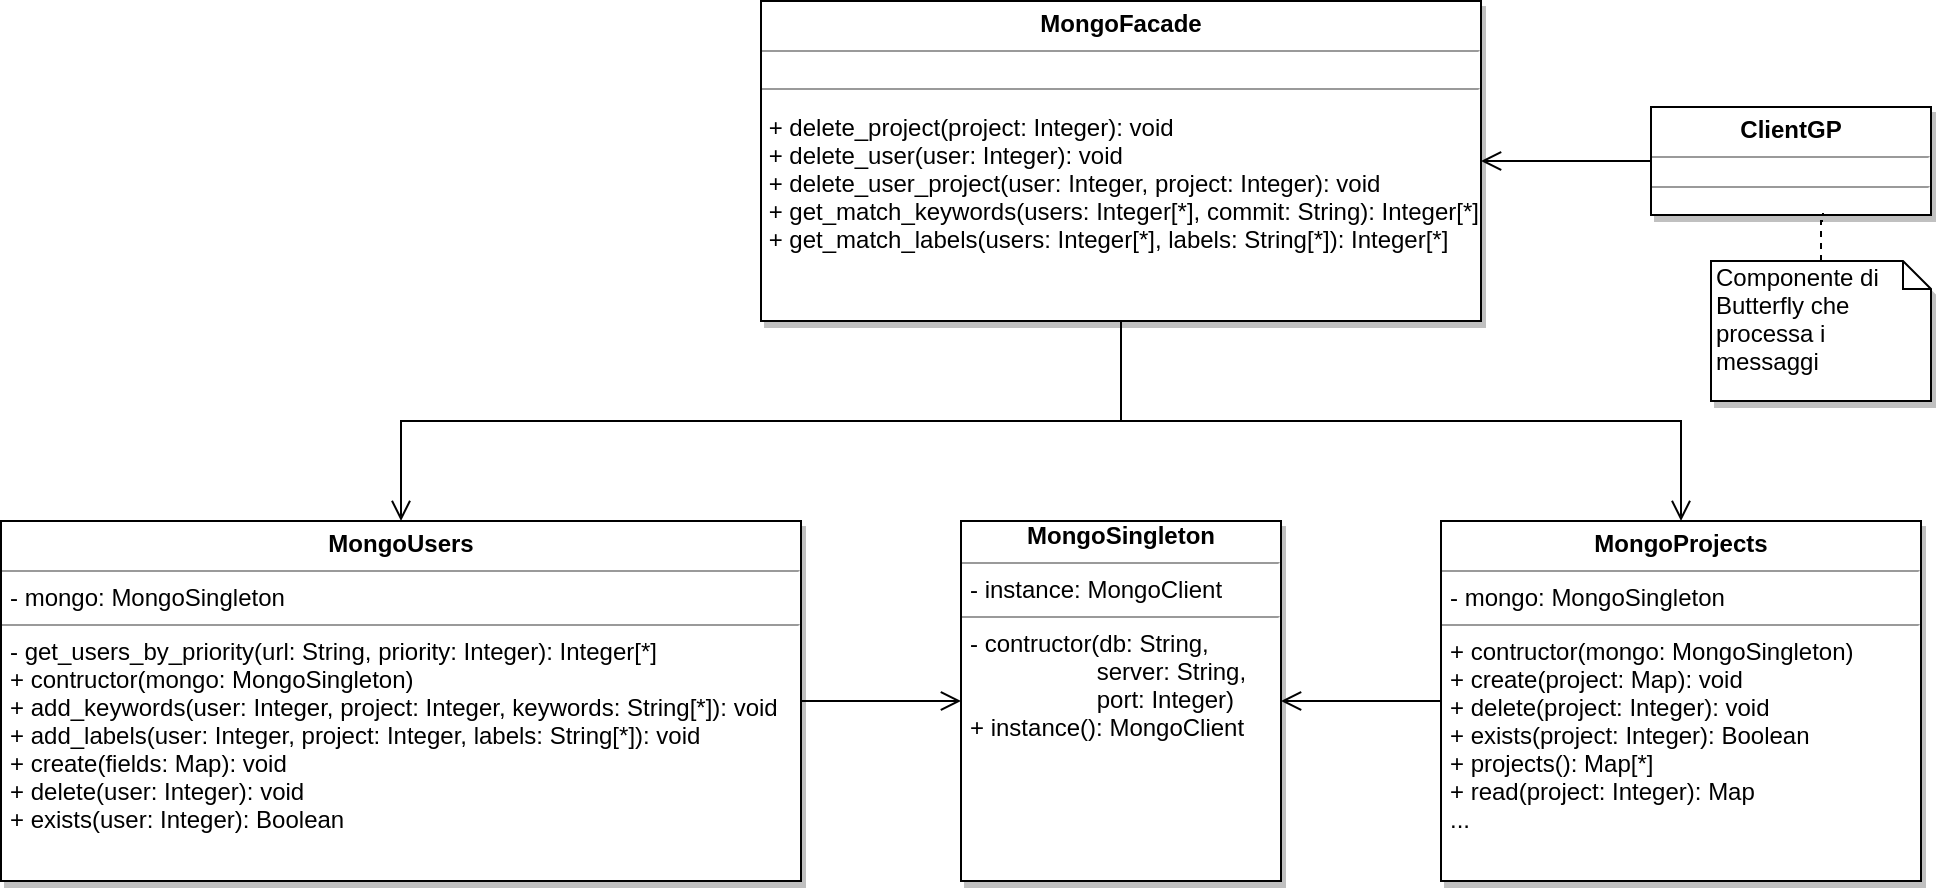
\includegraphics[width=\textwidth]{img/GP-Mongo.png}\\
        \caption{Interazione con MongoDB del Gestore Personale}
        \label{fig:GP-Mongo}
    \end{figure}

    Per quanto riguarda il database, abbiamo una classe singleton che permette al nostro sistema di avere un'unica istanza della connessione con PyMongo.
    I metodi che agiscono sulla base di dati sono implementati nelle classi \texttt{MongoUser} e \texttt{MongoProject}, e sono suddivisi in base alle risorse di interesse.
    Tali classi vengono raccolte in un facade che espone solamente i metodi che servono verso l’esterno, per renderli più facilmente fruibili. \par
    Nella figura \ref{fig:GP-Mongo} vengono mostrate queste classi e le loro dipendenze.


\subsubsection{Controller e View}
Il controller recupera gli input che gli utenti inseriscono attraverso la View, le interpreta, per poi poterle elaborare correttamente, interagendo eventualmente con il database. Nel momento in cui cambiano i dati relativi agli utenti nel database il controller aggiorna la View.


    \paragraph{Diagramma delle classi}

    \begin{figure}[H]
        \centering
        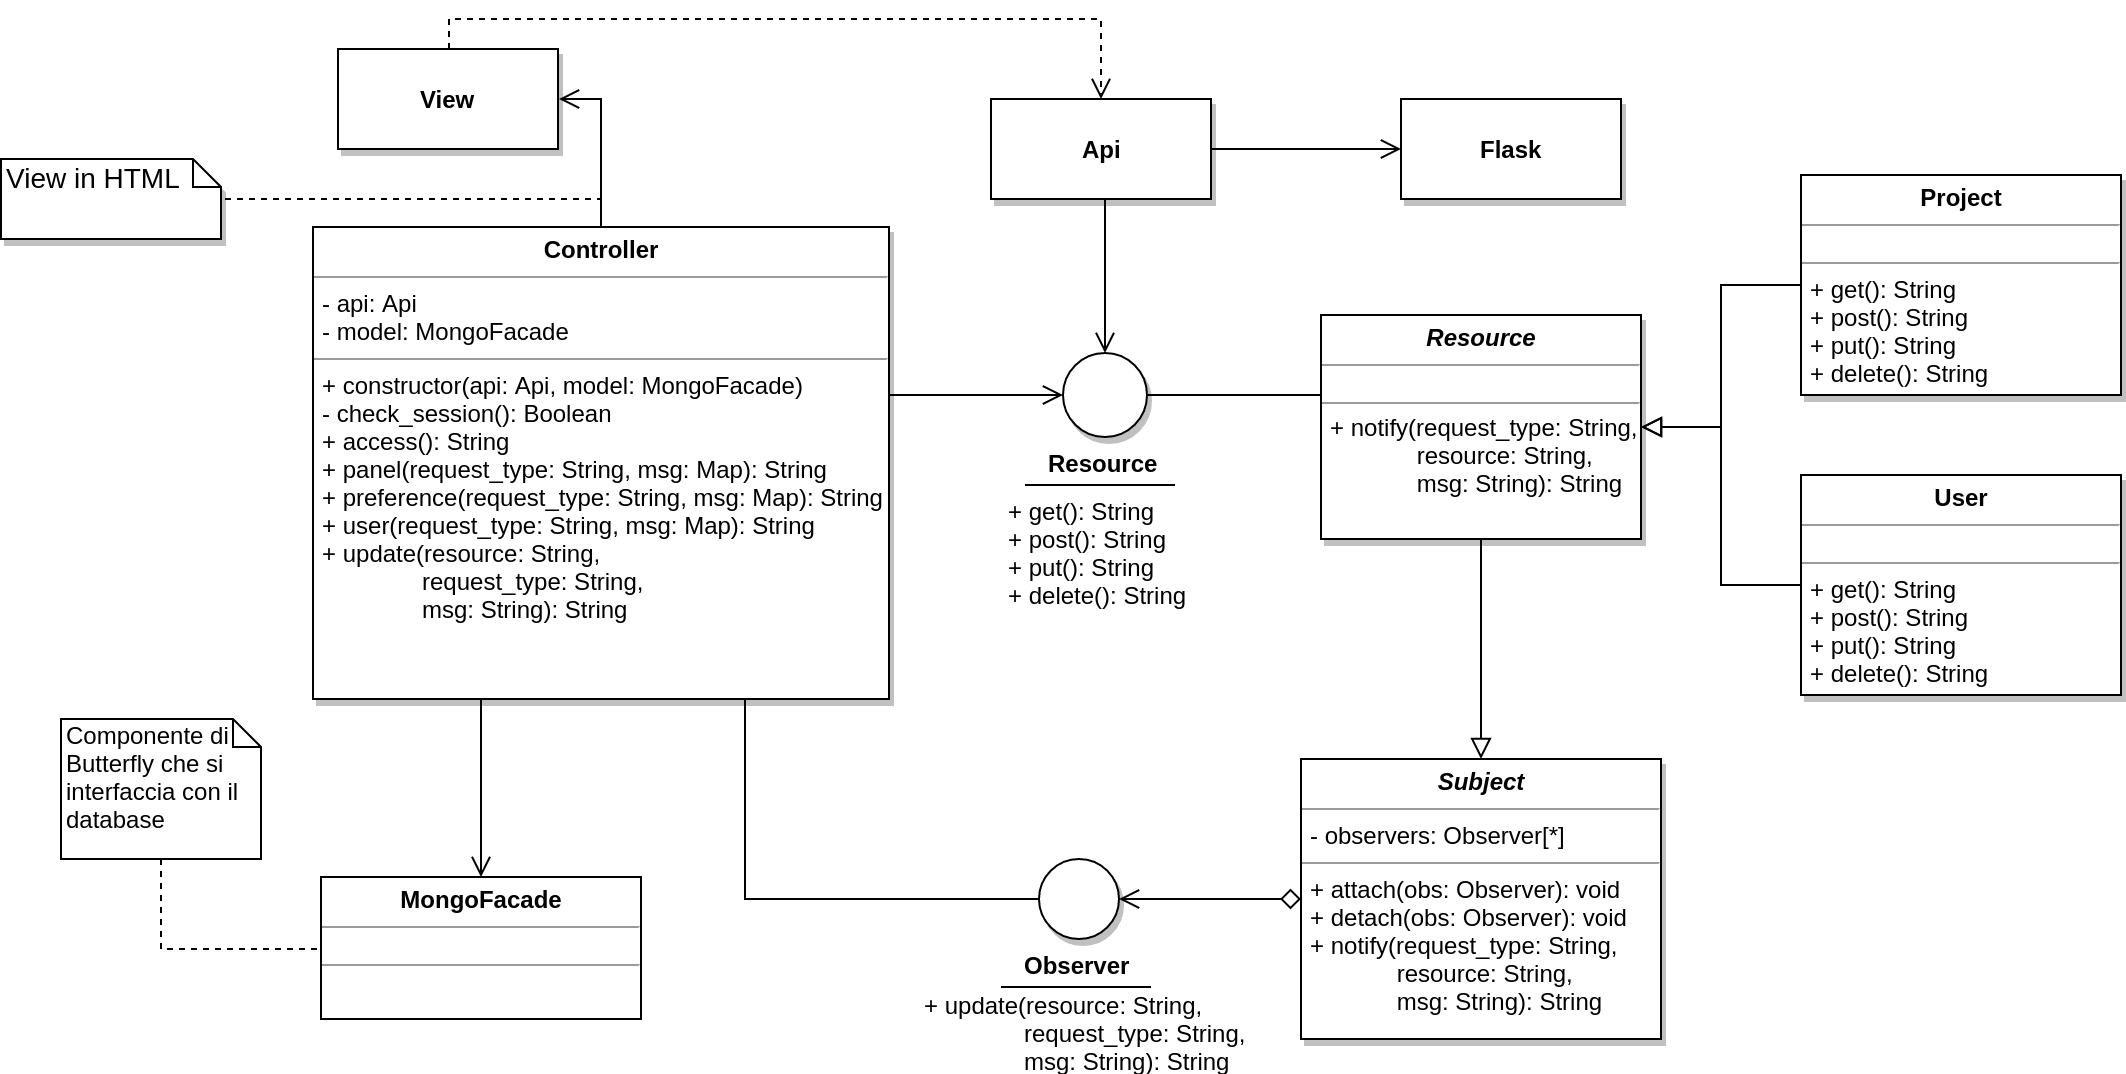
\includegraphics[width=\textwidth]{img/GP-View.png}\\
        \caption{Logica del Controller del Gestore Personale}
        \label{fig:GP-View}
    \end{figure}

    Il Controller del Gestore Personale serve per collegare la componente del Model con la componente View.
    Una volta istanziati il server Flask, l'API REST e MongoDB vengono passati al Controller che resta in ascolto.\par
    Quando arriva una richiesta dall'API REST o dalla View, il Controller esegue le dovute operazioni su MongoDB e restituisce una risposta alla vista di provenienza, in formato JSON se si tratta dell'API REST o in formato HTML se si tratta della view consultabile da browser Web.


\subsubsection{Client}
Il suo compito è quello di recuperare i messaggi inseriti in Kafka dai Producer GitLab e Redmine attraverso un Consumer fittizio, analizzare il messaggio, associargli il destinatario corretto e inserirlo nella coda di Kafka appropriata (di Telegram o Email) attraverso un Producer fittizio.

\newpage
Per analizzare il messaggio il Client opera in questo modo:

\begin{figure}[H]
    \centering
    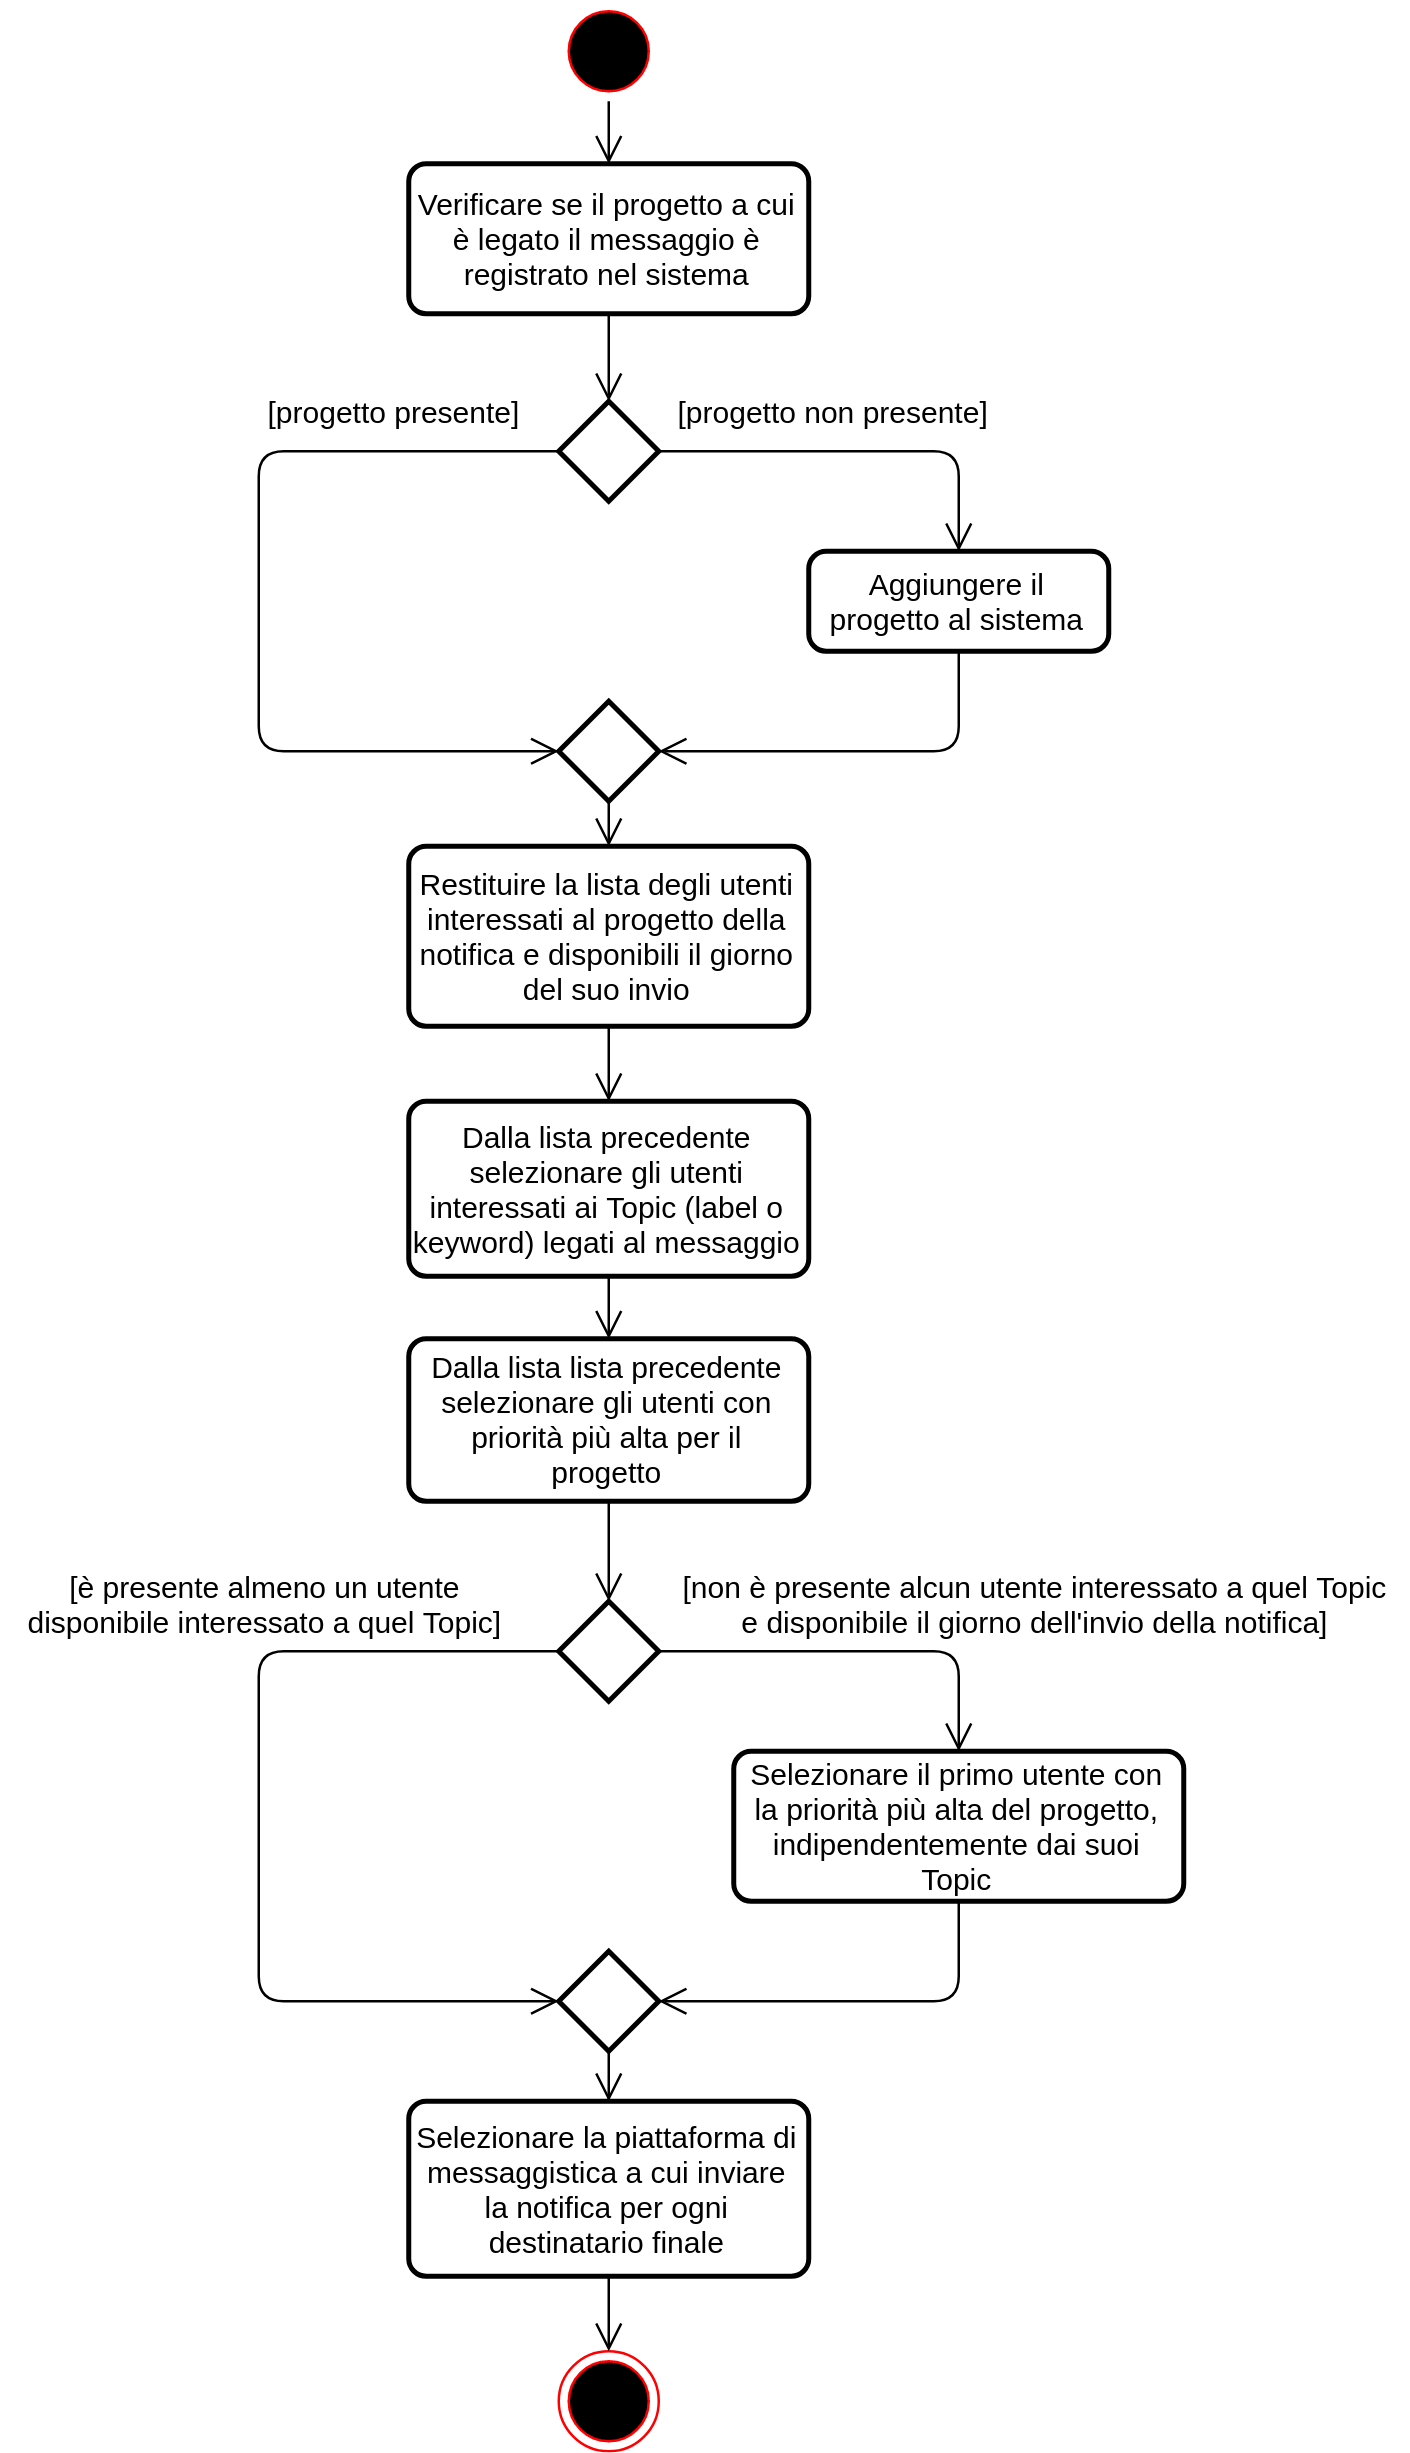
\includegraphics[width=0.80\textwidth]{img/Client_attivita.png}\\
    \caption{Diagramma di attività del Client}
    \label{fig:GP-Processor-attività}
\end{figure}

    \paragraph{Diagramma delle classi}

    \begin{figure}[H]
        \centering
        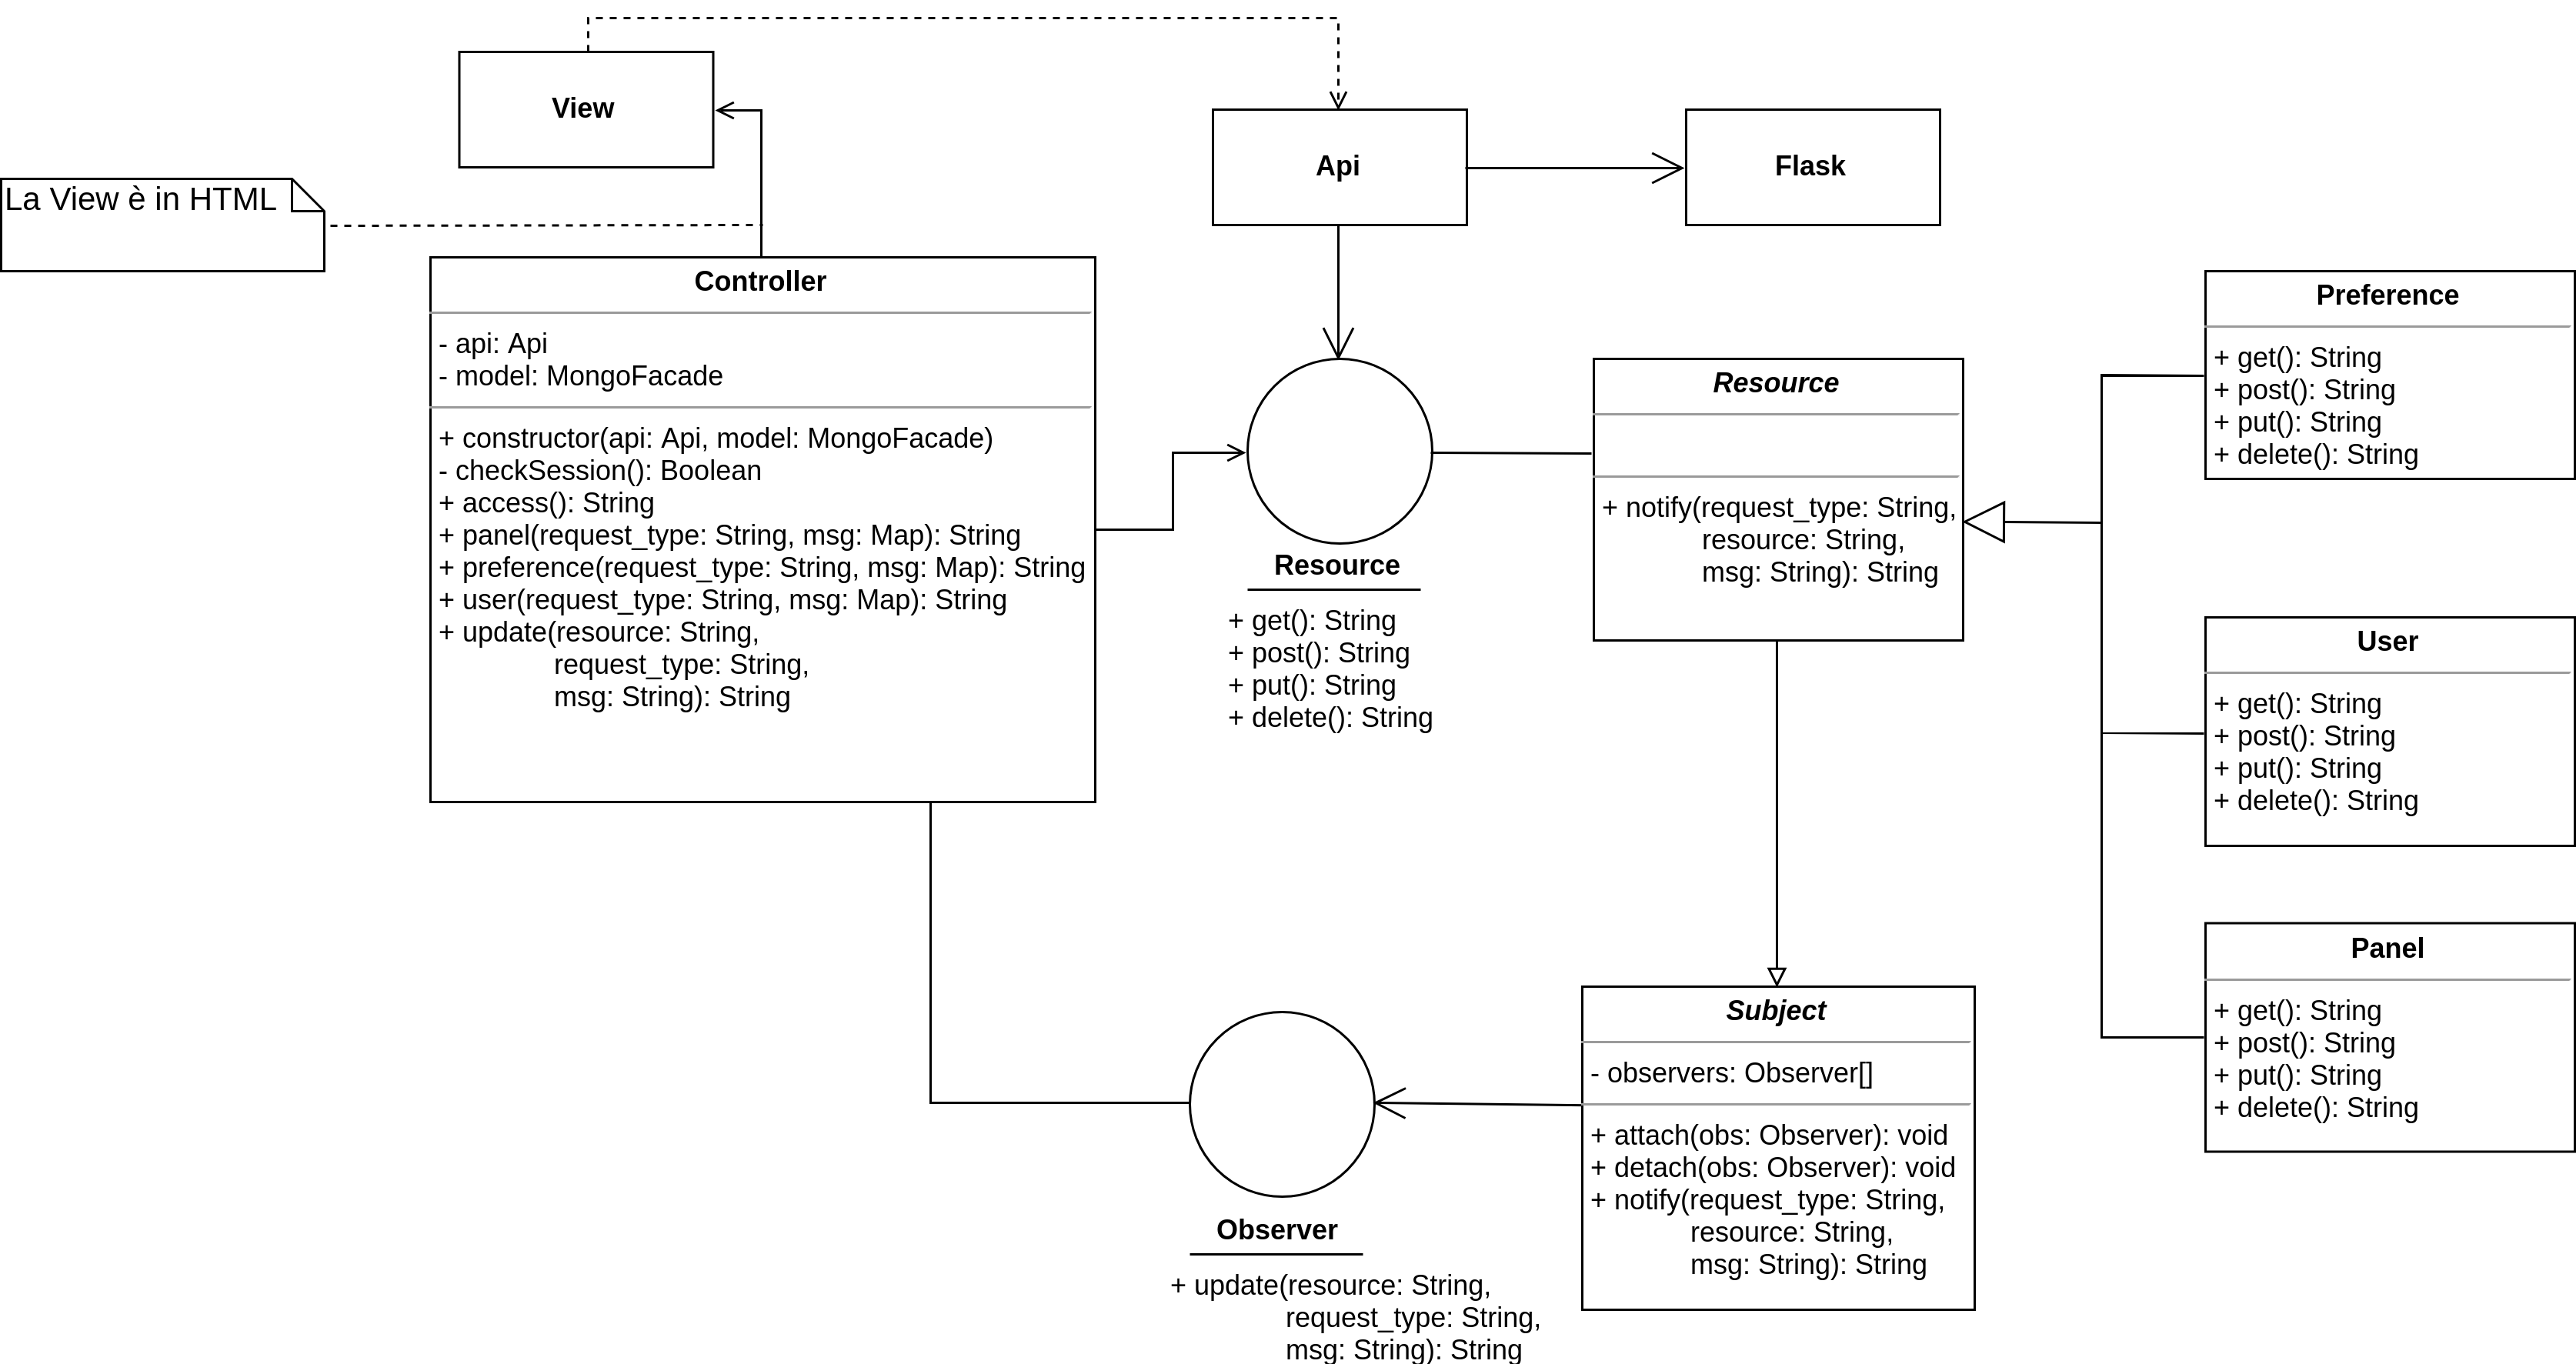
\includegraphics[width=\textwidth]{img/GP-Processor.png}\\
        \caption{Message processor del Gestore Personale}
        \label{fig:GP-Processor}
    \end{figure}

    Il Gestore Personale usa ora \texttt{ClientGP} che si interfaccia con Kafka attraverso \texttt{KafkaProducer} e \texttt{KafkaConsumer}, e per elaborare i messaggi che riceve crea un'implementazione di Processor. Questa, in base alle informazioni nel messaggio ricevuto, indica qual è il destinatario e attraverso quale applicazione notificarlo interrogando il database con \texttt{MongoFacade}.

\subsection{Consumers}
Il Consumer è il componente finale del sistema \progetto. Esso resta in ascolto della sua coda specifica di Kafka per applicativo (e.g. telegram, email).
Si occupa di inoltrare il messaggio al destinatario finale.

Al momento della stesura di questo manuale, i Consumer implementati sono due:

\begin{itemize}
    \item TelegramConsumer
    \item EmailConsumer
\end{itemize}

L'algoritmo di ascolto dei messaggi è identico per ogni Consumer: come per i Producer, abbiamo utilizzato
Template Method per l'implementazione di \texttt{listen()}.
Le classi concrete avranno esclusivamente il compito di implementare il metodo \texttt{send()}, il quale invierà il messaggio
al destinatario finale tramite le API dell'applicativo su cui il Consumer è basato.


\subsubsection{TelegramConsumer}
Nel seguente diagramma di sequenza è possibile vedere il flusso di esecuzione che parte dalla ricezione del messaggio dalla coda \textit{telegram}
di Kafka all'invio del messaggio all'utente finale su Telegram.

\paragraph{Diagramma dei package}

Il TelegramConsumer ha due dipendenze esterne:
\begin{itemize}
    \item \texttt{KafkaConsumer} dalla libreria esterna \texttt{kafka-python}: offre le funzionalità di ascolto
        di una o più code specifiche. È costruito su di esso un adapter, per adattare \texttt{KafkaConsumer} alle funzionalità
        di \texttt{Consumer}.
    \item Package \texttt{requests}: effettua le richieste POST e poter inviare i messaggi tramite l'API di Telegram
        al destinatario finale.
\end{itemize}

\begin{figure}[H]
    \centering
    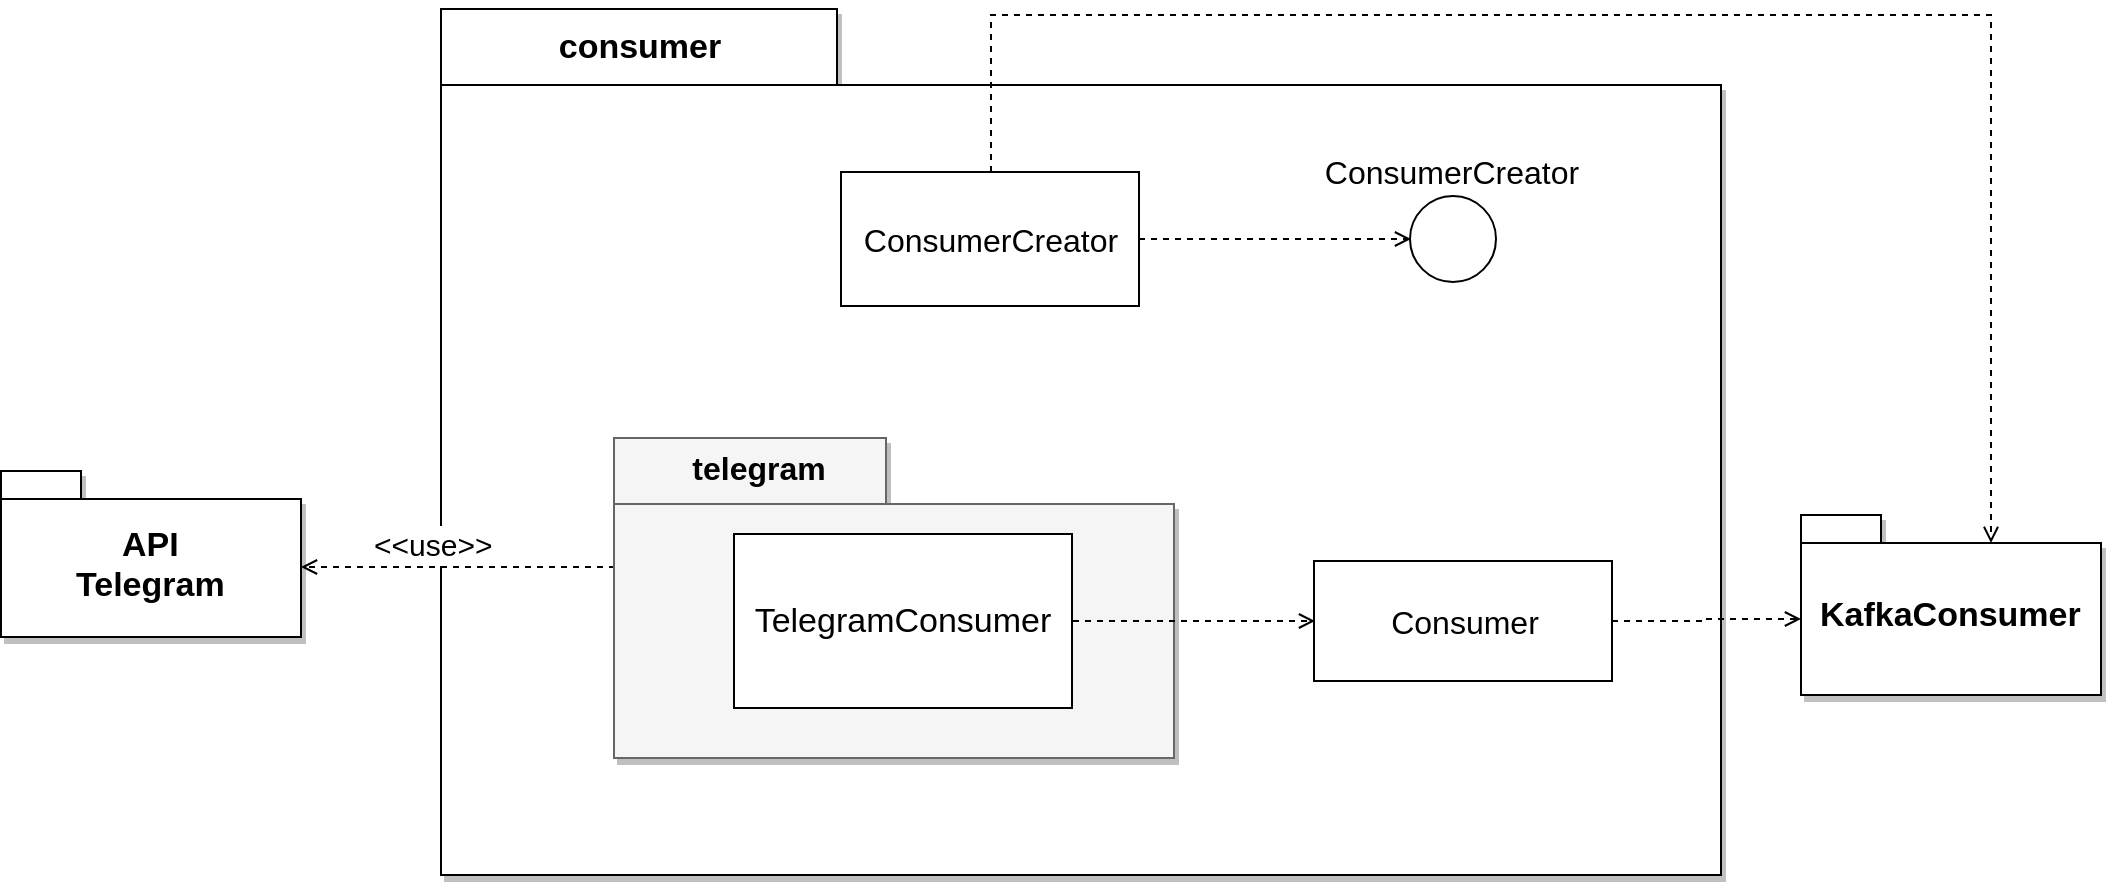
\includegraphics[width=\textwidth]{img/Package-TelegramConsumer.png}\\
    \caption{Diagramma dei package di TelegramConsumer}
    \label{fig:GP-Kafka}
\end{figure}

\paragraph{Diagramma delle classi}

Il metodo \texttt{format()} costruisce il testo del messaggio finale utilizzando il formato \gloss{markdown} specifico per Telegram.

\begin{figure}[H]
    \centering
    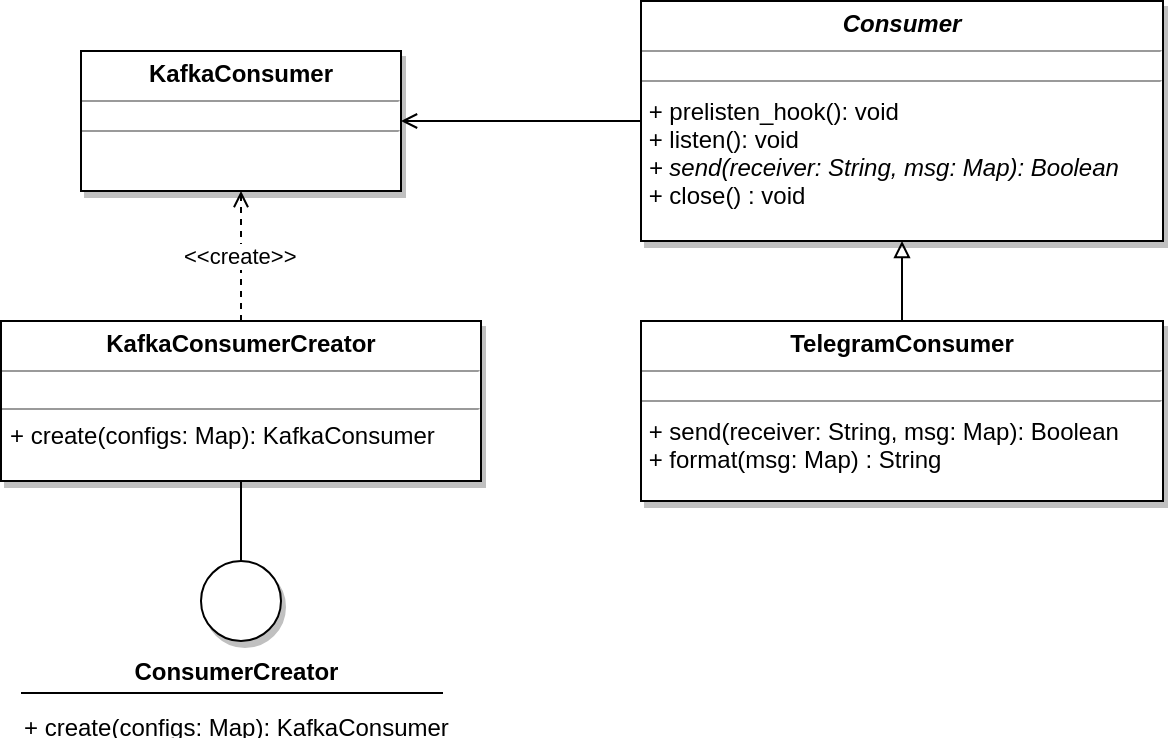
\includegraphics[width=0.8\textwidth]{img/Consumers-TelegramConsumer.png}\\
    \caption{Diagramma delle classi di TelegramConsumer}
    % \label{fig:GP-Kafka}
\end{figure}


\subsubsection{EmailConsumer}
\paragraph{Diagramma dei package}

L'EmailConsumer ha due dipendenze esterne:
\begin{itemize}
    \item \texttt{KafkaConsumer} della libreria esterna \texttt{kafka-python}: offre le funzionalità di ascolto dei messaggi
        proveniente da una o più code specifiche. È costruito su di esso un adapter, per adattare le funzionalità di \texttt{KafkaConsumer} a
        \texttt{Consumer}.
    \item \texttt{SMTP} della libreria esterna \texttt{smtplib}: server e-mail che, dopo aver effettuato il login,
        invia al destinatario una mail contenente il messaggio finale.
\end{itemize}

\begin{figure}[H]
    \centering
    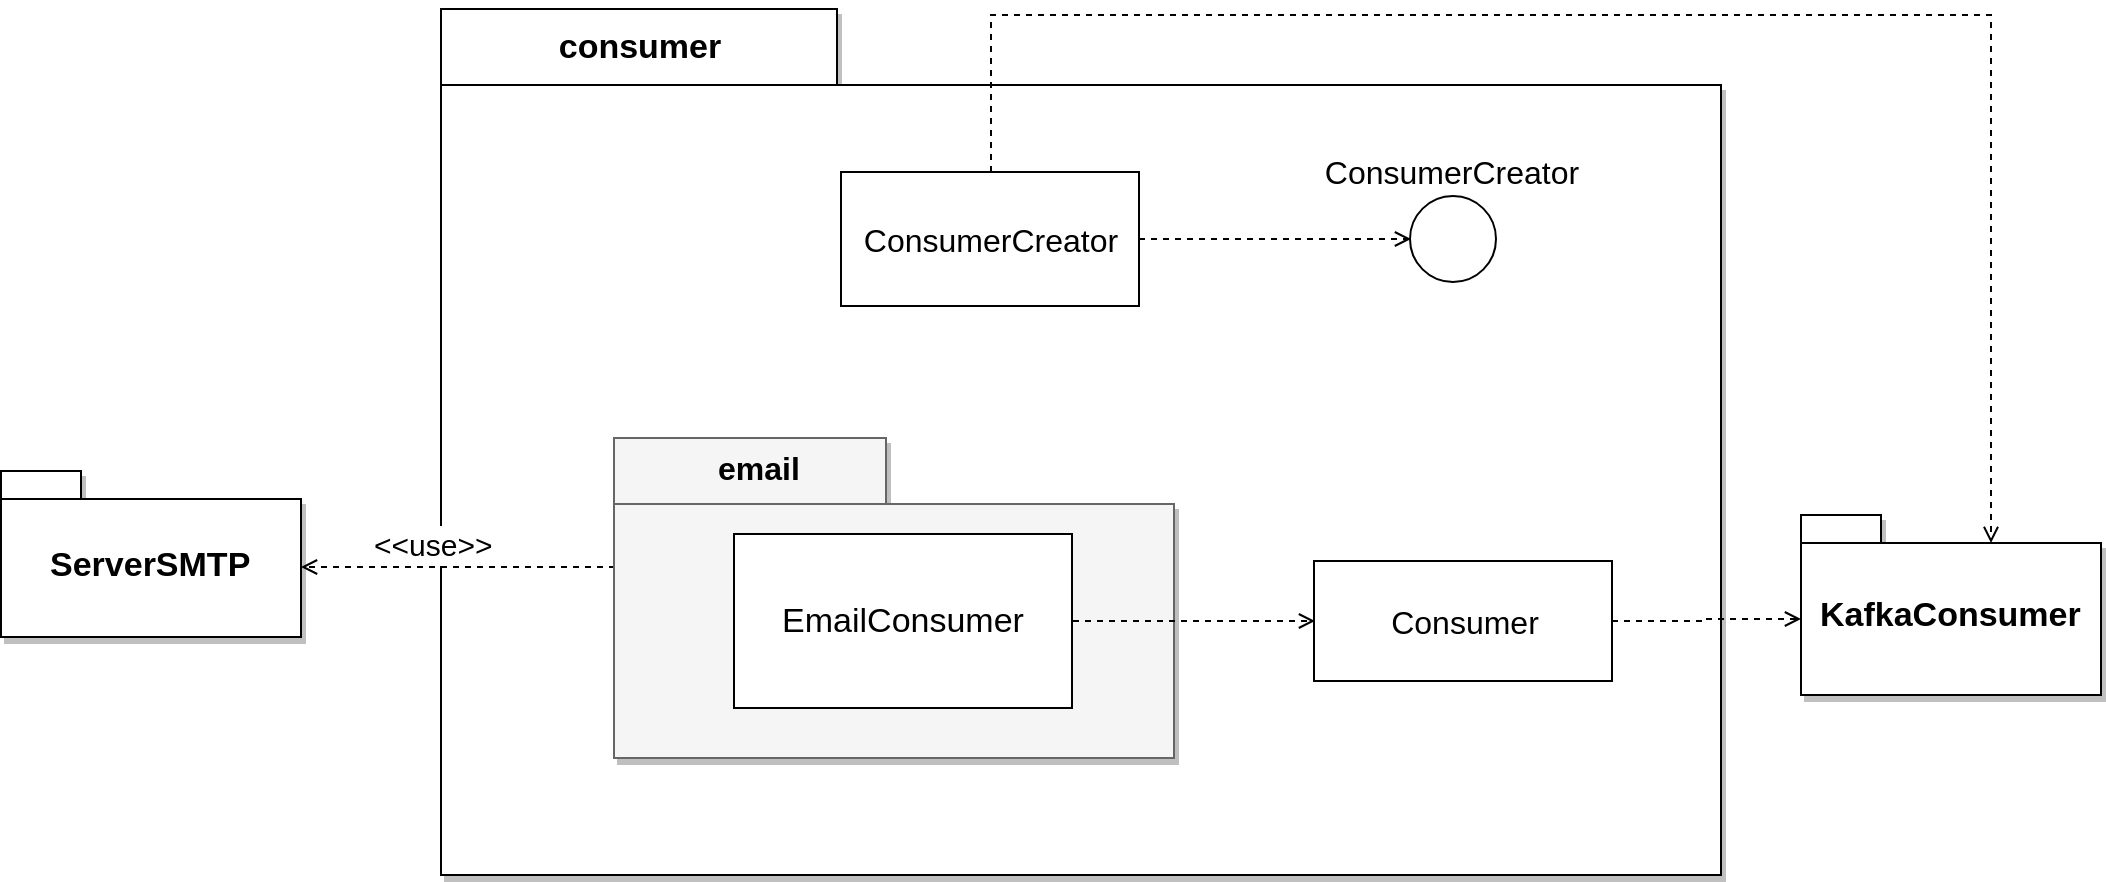
\includegraphics[width=\textwidth]{img/Package-EmailConsumer.png}\\
    \caption{Diagramma dei package di EmailConsumer}
    \label{fig:consumer}
\end{figure}


\paragraph{Diagramma delle classi}

\begin{itemize}
    \item Il metodo \texttt{format\_html()} costruisce il testo del messaggio finale in formato HTML
    \item Il metodo \texttt{format()} costruisce il testo per il messaggio senza i tag HTML, in caso il client mail del ricevente non sia in grado
        di interpretare tale linguaggio
\end{itemize}

\begin{figure}[H]
    \centering
    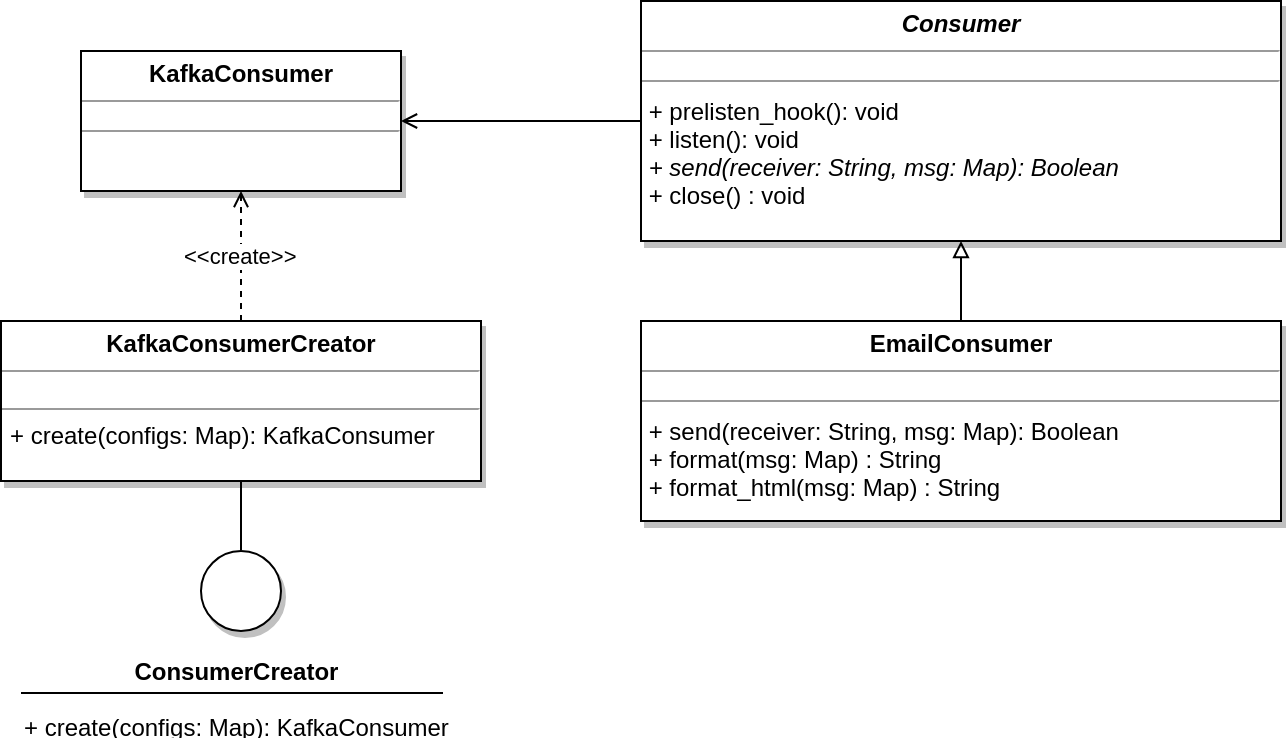
\includegraphics[width=0.8\textwidth]{img/Consumers-EmailConsumer.png}\\
    \caption{Diagramma delle classi di EmailConsumer}
    % \label{fig:GP-Kafka}
\end{figure}


\subsection{Impostazioni dei vari componenti}

Per fare in modo che tutti i componenti vengano istanziati con i determinati parametri che permettano la giusta comunicazione tra le componenti,
ci sono dei file di configurazioni che contengono per esempio il token del bot Telegram, l'email e la password per accedere al server Email. Queste configurazioni
sono contenute nelle variabili d'ambiente descritte nel \MSd, oppure nei file \texttt{``config.json''} contenuti nelle cartelle dei vari componenti (e.g. producer,
consumer ecc.).

\subsection{Interazione tra i componenti}

Vedendo \progetto\ ad alto livello, si possono identificare sei componenti. Redmine e GitLab, per comunicare con i relativi Producer, utilizzano dei webhook in formato JSON,
mettendosi in ascolto su determinate porte utilizzando il webserver Flask. Per quanto riguarda la comunicazione tra i Producer e Kafka utilizziamo delle istanze
di KafkaProducer. Per far comunicare Kafka con i vari Consumer utilizziamo istanze di KafkaConsumer. Nell'ultimo passo, quello che riguarda i Consumer e le applicazioni finali, quali Telegram e Email, usiamo le API messe a disposizione dagli applicativi.

    \section{Estendibilità}

\subsection{Aggiungere un Webhook}

Per aggiungere una nuova tipologia di Webhook, è sufficiente estendere l'interfaccia \texttt{Webhook}
e un eventuale \texttt{WebhookFactory} in caso si tratti di una nuova applicazione.

\begin{figure}[H]
    \centering
    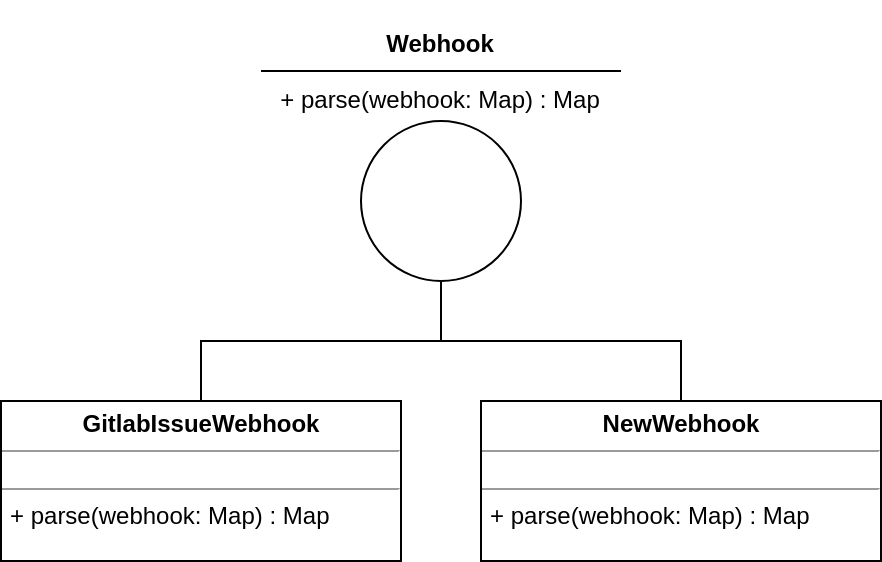
\includegraphics[width=0.7\textwidth]{img/EstensioneWebhook.png}\\
    \caption{Estendere un Webhook}
\end{figure}


\begin{figure}[H]
    \centering
    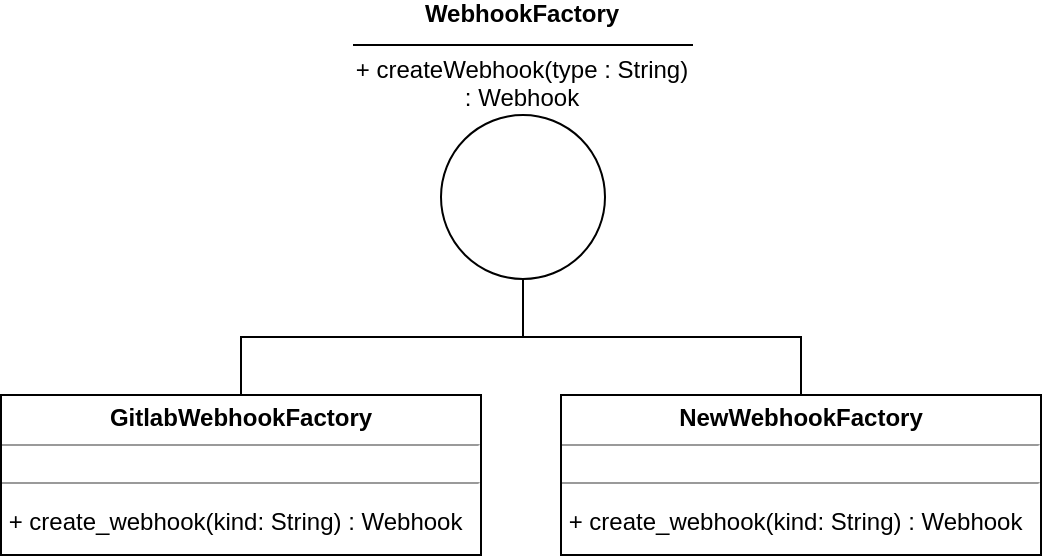
\includegraphics[width=0.7\textwidth]{img/EstensioneFactory.png}\\
    \caption{Estendere una Factory}
\end{figure}

    \section{Test} \label{test}

Tale sezione ha lo scopo di spiegare il funzionamento, lo scopo e i risultati dei vari tipi di test proposti dal modello a V.

\subsection{Modello a V} \label{sezionemodelloV}
Il modello a V descrive in modo sintetico il ciclo di vita della realizzazione del software, partendo dalla sua progettazione fino alla sua consegna al cliente escludendo la fase di manutenzione.

Lo scopo del modello a V è quello di mostrare quali tipi di test accompagnano ogni fase del ciclo e di come anche questi siano propedeutici l'uno dall'altro.

\begin{figure}[H]
	\centering
	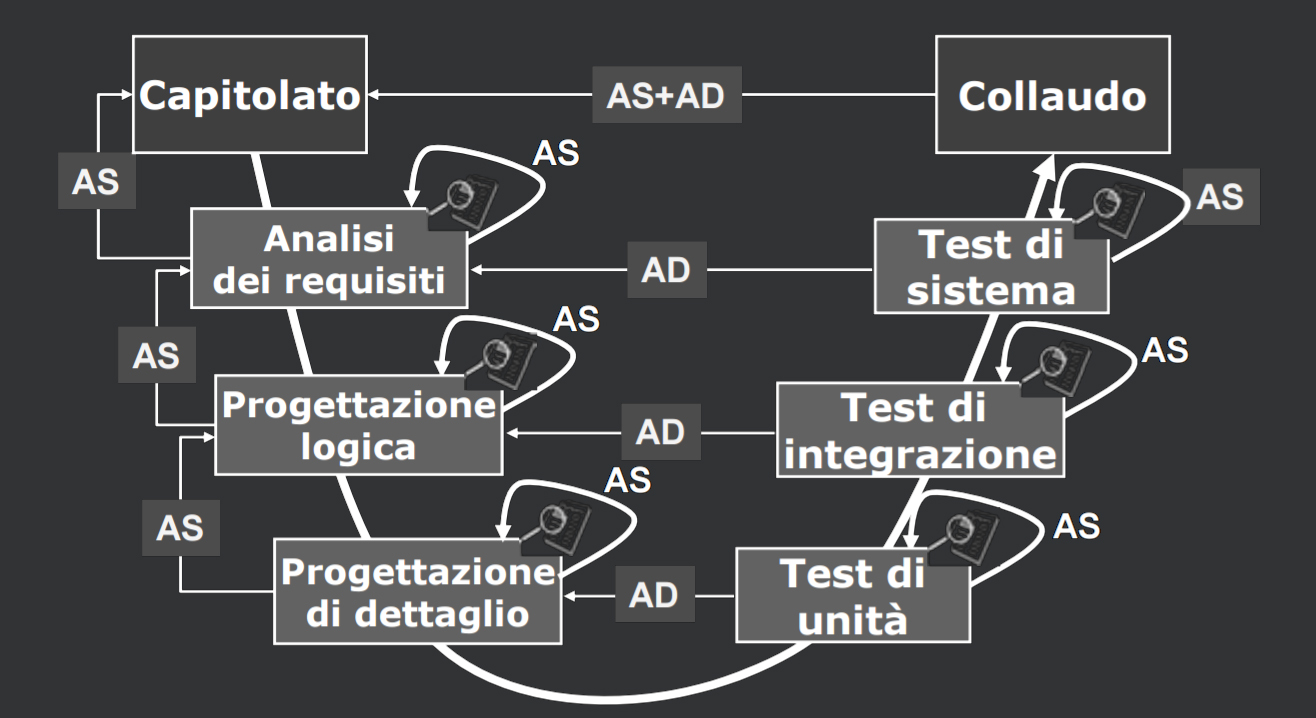
\includegraphics[width=0.8\textwidth]{img/modellov-sweki.jpg}
	\label{img:vmodel}
	\caption{Modello a V\protect\footnotemark}
\end{figure}

\footnotetext{Vedere modello a V in \S\ref{riferimenti informativi}}



\subsection{Classificazione e stuttura dei test} \label{classificazionetest}
Ogni test viene identificato univocamente dal seguente codice:

\begin{center}
	\texttt{T[Tipo][ID]}
\end{center}

\begin{itemize}
	\item \textbf{T}: si riferisce a "Test".
	\item \textbf{Tipo}: la tipologia a cui il test appertiene che, seguendo il modello a V, sono:
	\begin{itemize}
		\item \textbf{V}: validazione. %è la stessa cosa di collaudo e di accettazione??
		\item \textbf{S}: sistema
		\item \textbf{I}: integrazione.
		\item \textbf{U}: unità.
		\end{itemize}
	%per la corrispondenza con i requisiti, non vanno bene le "tre cifre"
	\item \textbf{ID}: numero incrementale che rispetta una struttura gerarchica.
\end{itemize}

% COLORI 
\newcommand{\TNI}{{\color{gray}\textbf{NI}}}
\newcommand{\TI}{{\color{blue}\textbf{I}}}
\newcommand{\TNS}{{\color{red}\textbf{NS}}}
\newcommand{\TS}{{\color{green}\textbf{S}}}

Le tabelle che raccolgno i test di una determinata tipologia presentano i campi:
\begin{itemize}
	\item \textbf{Codice}: comprendente il codice identificativo del test.
	\item \textbf{Test}: descrive cosa il test deve verificare.
	\item \textbf{Stato}: indica lo stato del test e può essere:
	\begin{itemize}
		\item \TNI: non implementato.
		\item \TI: implementato ma non ancora avviato.
		\item \TNS: avviato e fallito.
		\item \TS: avviato e superato.
	\end{itemize}	
\end{itemize}



\subsection{Test di validazione} \label{testvalidazione} % TODO
Tipo di test da determinare in parallelo con la comprensione del capitolato.
Come si può vedere dal modello a V, sono i primi tipi di test che vengono creati e saranno gli ultimi ad essere eseguiti prima della consegna del prodotto.

\newenvironment{VTtable}[1][1]{%
	\renewcommand*{\arraystretch}{#1}%
	\renewcommand\theadfont{\bfseries}%
	\oldtabularx%
}{\endoldtabularx}

\begin{table}[H]
	\begin{VTtable}[1.7]{\textwidth}{cXc}
		\textbf{Codice} & \textbf{Test} & \textbf{Stato} \\\toprule
		TV1 & Verfica la segnalazione dell' apertura di una issue da parte di Redmine:
		\begin{enumerate}
			\item Redmine apre una issue
			\item La segnalazione contiene tutti i campi di interesse
			\item Redmine invia la segnalazione
		\end{enumerate}
		& \TNI \\\midrule

		TV1 & Verifica l'inserimento di un nuovo utente:
		\begin{enumerate}
			\item Inserire nel gestore personale le seguenti informazioni del nuovo utente:
			\begin{itemize}
				\item Nome
				\item Cognome
				\item Contatto Telegram
				\item Contatto email
			\end{itemize}
			\item Conferma invio dei dati.
		\end{enumerate}
		& \TNI \\\midrule
		TV2 & Verifica  & \TNI \\\bottomrule
	\end{VTtable}
	\caption{Elenco dei test di validazione}
\end{table}

	\subsubsection{Tracciamento} \label{tracciamentovalidazione}

	\begin{table}[H]
		\centering
		{\def\arraystretch{1.4}
		\begin{tabularx}{\textwidth}{YY}
			\textbf{Codice} & \textbf{Requisito} \\
			\toprule
			TV1 & requisito da inserire \\
			TV2 & requisito da inserire \\
			\bottomrule\\
		\end{tabularx}}
		\caption{Elenco dei test in correlazioni con i requisiti.}
	\end{table}



\subsection{Test di sistema} \label{testsistema} %FIXME
Tipo di test da scegliere durante l'attività di analisi dei requisiti. Servono per svolgere la validazione del prodotto.

I test di sistema servono per testare l'intero prodotto, in particolare le sue specifiche tecniche e funzionali.
Per questo si creano dei test derivanti dai casi d'uso e dai requisiti funzionali presenti nell'\AdRd.

%Per ogni test vengono affrontati i seguenti punti:
%
%\begin{itemize}
%	\item \textbf{Scopo}: lo scopo del test che; il titolo del punto non verrà inserito nei paragrafi dei test. %TODO: WHAT??
%	\item \textbf{Procedura}: vengono descritti i passaggi da compiere per eseguire il test.
%	\item \textbf{Approvazione}: vengono descritte le condizioni affinché il test sia considerato superato.
%\end{itemize}
%
%Alcuni termini ed espressioni assumono il seguente significato:
%
%\begin{itemize}
%	\item \textbf{Piattaforma di messaggistica}: s'intende sempre Telegram ed email.
%	\item \textbf{Notifica}: s'intende una notifica in una delle piattaforme di messaggistica causata dall'applicazione.
%	\item \textbf{Topic}: s'intende l'insieme delle etichette delle issue di GitLab e Redmine e delle keyword presenti nei messaggi di commit notificati dai push di GitLab.
%	\item \textbf{Persona delegata}: s'intende l'utente a cui verranno inoltrate le notifiche nei giorni di indisponibilità dell'utente che sta usando l'applicazione. 
%\end{itemize}

		%\paragraph*{Accettazione}
		%Il nuovo utente deve comparire all'interno della lista degli utenti inseriti nell'applicazione.
	
	\subsubsection{TS002 Iscrizione ad una label, ad una piattaforma di messaggistica e apertura issue}
		Un utente quando s'iscrive ad una label, lo fa con l'intenzione di ricevere le notifiche inerenti solo a quella label provenienti da GitLab o Redmine e l'iscrizione alla piattaforma di messaggistica (Telegram o email) per scegliere dove ricevere tali notifiche.
		
		\paragraph*{Procedura}
			\begin{enumerate}
				\item Selezionare l'utente con cui si vuole usare l'applicativo.
				\item Selezionare la label da cui si vuole ricevere le notifiche. Dalle label è possibile capire quali notifiche derivano da Redmine e quali da GitLab.
				\item Selezionare Telegram o email per decidere in che piattaforma di messaggistica ricevere le notifiche della label.
				\item Aprire una issue da Gitlab se l'iscrizione è stata fatta da una label proveniente da GitLab, o aprire una issue da Redmine se l'iscrizione è stata fatta da una label proveniente da Redmine.
			\end{enumerate}
		
		\paragraph*{Accettazione}
		Alla piattaforma di messaggistica selezionata arriva una notifica dell'apertura della issue inerente al topic selezionato.
		
	\subsubsection{TS003 Iscrizione a una label, a una piattaforma di messaggistica e modifica issue}
		Come descritto nel test precedente, un utente può iscriversi a una label e a una piattaforma di messaggistica per ricevere una notifica.
		
		\paragraph*{Procedura}
			\begin{enumerate}
				\item Selezionare l'utente con cui si vuole usare l'applicativo.
				\item Selezionare la label da cui si vuole ricevere le notifiche. Dalla label è possibile capire quali derivano da Redmine e quali da GitLab.
				\item Selezionare Telegram o email per decidere in che piattaforma di messaggistica ricevere le notifiche delle label.
				\item Selezionare su Redmine, se ci si è iscritti ad una label di Redmine, o su GitLab, se ci si è inscritti ad una label su GitLab, una issue già aperta e modificarla in termini di label o titolo della issue.
				\item Se tra i campi modificati nella issue ci sono anche le label, iscriversi nel gestore personale alla label della issue modificata.
			\end{enumerate}
		
		\paragraph*{Accettazione}
		La modifica del titolo o delle label di una issue di Redmine o GitLab comporta l'invio della notifica a tutti gli iscritti alle nuove label, se queste sono cambiate, altrimenti agli iscritti delle solite label se è cambiato solo il titolo della issue. La modifica di qualsiasi altro campo non comporta l'invio di una notifica.
		
	\subsubsection{TS004 Disiscrizione da una label}
		La disiscrizione ad una label deve terminare la notifica delle segnalazioni legate a quella label.
		
		\paragraph*{Procedura}
			\begin{enumerate}
				\item Selezionare l'utente con cui si vuole usare l'applicativo.
				\item Disiscriversi da una label a cui precedentemente si era iscritti.
				\item Aprire o modificare una issue da Redmine o GitLab con la label da cui ci si è disiscritti precedentemente.
			\end{enumerate}
		
		\paragraph*{Accettazione}
		Una volta disiscritti ad una label non vengono più ricevute notifica riguardanti quella label.
		
	\subsubsection{TS005 Aggiunta di una keyword, iscrizione ad una piattaforma di messaggistica e push di Gitlab}
		Per ricevere le notifiche dei push di GitLab è possibile selezionare delle keyword che possono essere presenti nei messaggi di commit.
		
		\paragraph*{Procedura}
		\begin{itemize}
			\item Selezionare l'utente con cui si vuole usare l'applicativo.
			\item Aggiungere una keyword nel gestore personale.
			\item Effettuare un push su Gitlab dove il messaggio di commit contiene la keyword appena inserita.
		\end{itemize}
	
		\paragraph*{Accettazione}
		L'utente le notifiche dei push che nel loro messaggio di commit contengo la keyword aggiunta.
	
	\subsubsection{TS006 Rimozione di una keyword}
		La rimozione di una delle keyword aggiunta precedentemente evita di ricevere la notifica dei push di GitLab con il messaggio di commit con la keyword rimossa.
		
		\paragraph*{Procedura}
			\begin{enumerate}
				\item Selezionare l'utente con cui si vuole usare l'applicativo.
				\item Rimuovere una delle keyword selezionate in precedenza.
				\item Effettuare un push su GitLab dove il messaggio di commit contiene la keyword appena rimossa.
			\end{enumerate}
		
		\paragraph*{Accettazione}
		Non arrivano le notifiche dei push di Gitlab in cui nel messaggio di commit è presente la keyword appena rimossa.
		
	\subsubsection{TS007 Rimozione di una piattaforma di messaggistica}
		Come per il test precedente, anche rimuovendo una piattaforma di messaggistica (Telegram o email), le notifiche a quella piattaforma non dovrebbero più arrivare.
		
		\paragraph*{Procedura}
		\begin{enumerate}
			\item Selezionare l'utente con cui si vuole usare l'applicativo.
			\item Deselezionare una piattaforma di messaggistica precedentemente selezionata
			\item Creare o modificare una issue da Redmine o Gitlab, oppure effettuare un \gloss{push}. 
		\end{enumerate}
	
		\paragraph*{Accettazione}
		Dopo aver aperto una issue o effettuato un push da Gitlab o Redmine, non si ricevono più notifiche dalle piattaforme di messaggistica rimosse.
		
	\subsubsection{TS008 Aggiunta della persona delegata e dei giorni di indisponibilità}
		All'interno del gestore personale è possibile indicare i giorni di calendario in cui si è irreperibili ed è possibile selezionare una persona a cui inoltrare le notifiche che arrivano nei giorni selezionati.
		
		\paragraph*{Procedura}
			\begin{enumerate}
				\item Selezionare l'utente con cui si vuole usare l'applicativo.
				\item Aggiungere nel gestore personale il giorno di esecuzione del test come giorno di indisponibilità in cui non si vogliono ricevere notifiche dall'applicativo.
				\item Aggiungere, tra gli utenti inseriti nell'applicazione, l'utente a cui inoltrare le notifiche nei giorni di indisponibilità.
				\item Creare o modificare una issue da Redmine o Gitlab, oppure effettuare un \gloss{push}. 
			\end{enumerate}
		
		\paragraph*{Accettazione}
		La persona delegata riceve la notifica del messaggio che sarebbe dovuta arrivare all'utente che non è disponibile.
		
	\subsubsection{TS009 Rimozione giorni di indisponibilità}
		Nel momento in cui si rimuovono i giorni in cui ci si considera non reperibili, le notifiche dei topic a cui ci si è iscritti tornano ad essere inviate.
		
		\paragraph*{Procedura}
			\begin{enumerate}
				\item Selezionare l'utente con cui si vuole usare l'applicativo.
				\item Deselezionare tra i giorni di irreperibilità il giorno di esecuzione del test (se il giorno è già selezionato, selezionarlo e poi deselezionarlo).
				\item Effettuare un push da GitLab oppure aprire o modificare una issue su Redmine o GitLab.
			\end{enumerate}
		
		\paragraph*{Accettazione}
		L'utente selezionato ricomincia a ricevere notifiche.

	\subsubsection{Tracciamento}

	\begin{table}[H]
		\centering
		{\def\arraystretch{1.4}
		\begin{tabularx}{0.7\textwidth}{YY}
			\textbf{Codice} & \textbf{Requisito} \\
			\toprule
			TS1 & requisito da inserire \\
			TS2 & requisito da inserire \\
			\bottomrule\\
		\end{tabularx}}
		\caption{Elenco dei test in correlazioni con i requisiti.}
	\end{table}
		


\subsection{Test d'integrazione} \label{testintegrazione}

\newcounter{nTI}
\newcounter{subnTI}[nTI]
\newcommand{\newTI}[2]{\stepcounter{nTI}TI\thenTI & #1 & #2 \\}
\newcommand{\subTI}[2]{\stepcounter{subnTI}TI\thenTI.\thesubnTI & #1 & #2 \\}


\begin{table}[H]
	\begin{paddedtablex}[1.7]{\textwidth}{cXc}
		\textbf{Codice} & \textbf{Test} & \textbf{Stato} \\\toprule
		\newTI{Verifica l'integrazione tra Webhook di Gitlab e Producer Gitlab}{\TNI}
		\newTI{Verifica l'integrazione tra Webhook di Redmine e Producer Redmine}{\TNI}
		\newTI{Verifica l'integrazione del Cosumer Telegram con il bot Telegram}{\TNI}
		\newTI{Verifica l'integrazione del Consumer Email con il server Email}{\TNI}
		\newTI{Verifica l'integrazione di un file JSON con le componenti Producer}{\TNI}
			\subTI{Verifica l'integrazione di un file JSON con il Producer Gitlab}{\TNI}
			\subTI{Verifica l'integrazione di un file JSON con il Producer Redmine}{\TNI}
		\newTI{Verifica l'integrazione di un file JSON con le componenti Consumer}{\TNI}
			\subTI{Verifica l'integrazione di un file JSON con il Consumer Telegram}{\TNI}
			\subTI{Verifica l'integrazione di un file JSON con il Consumer Emai}{\TNI}
		\newTI{Verifica l'integrazione di Kafka con le componenti Producer e Consumer}{\TNI}
		\newTI{Verifica l'integrazione di Kafka nel Producer Gitlab}{\TNI}
		\newTI{Verifica l'integrazione di Kafka nel Producer Redmine}{\TNI}
		\newTI{Verifica l'integrazione di Kafka nel Cosumer Telegram}{\TNI}
		\newTI{Verifica l'integrazione di Kafka nel Consumer Email}{\TNI}
		\newTI{Verifica l'integrazione del database MONGODB con l'interfaccia del Gestore Personale}{\TNI}

		% TI1 & Verifica l'integrazione tra Webhook di Gitlab e Producer Gitlab & \TNI \\
		% TI2 & Verifica l'integrazione tra Webhook di Redmine e Producer Redmine & \TNI \\
		% TI3 & Verifica l'integrazione del Cosumer Telegram con il bot Telegram & \TNI \\
		% TI4 & Verifica l'integrazione del Consumer Email con il server mail & \TNI \\
		% TI5 & Verifica l'integrazione di un file JSON con le componenti Producer e Consumer & \TNI \\
		% TI5.1 & Verifica l'integrazione di un file JSON con il Producer Gitlab & \TNI \\
		% TI5.2 & Verifica l'integrazione di un file JSON con il Producer Redmine & \TNI \\
		% TI5.3 & Verifica l'integrazione di un file JSON con il Consumer Telegram & \TNI \\
		% TI5.4 & Verifica l'integrazione di un file JSON con il Consumer Email & \TNI \\
		% TI6 & Verifica l'integrazione di Kafka con le componenti Producer e Consumer & \TNI \\
		% TI6.1 & Verifica l'integrazione di Kafka nel Producer Gitlab & \TNI \\
		% TI6.2 & Verifica l'integrazione di Kafka nel Producer Redmine & \TNI \\
		% TI6.3 & Verifica l'integrazione di Kafka nel Cosumer Telegram & \TNI \\
		% TI6.4 & Verifica l'integrazione di Kafka nel Consumer Email & \TNI \\
		% TI7 & Verifica l'integrazione del database MONGODB con l'interfaccia del Gestore Personale & \TNI \\
		\bottomrule\\
	\end{paddedtablex}
	\caption{Elenco dei test d'integrazione.}
\end{table}

	\subsubsection{Tracciamento} \label{tracciamentointegrazione}

	\begin{table}[H]
		\centering
		{\def\arraystretch{1.4}
		\begin{tabularx}{0.7\textwidth}{YY}
			\textbf{Codice} & \textbf{Componente} \\
			\toprule
			TI1 & Producer Gitlab \\
			TI2 & Producer Redmine \\
			TI3 & Consumer Telegram \\
			TI4 & Consuer Email \\
			TI5 & Producer/Consumer \\
			TI5.1 & Producer Gitlab \\
			TI5.2 & Producer Redmine \\
			TI5.3 & Consumer Telegram \\
			TI5.4 & Consuer Email \\
			TI6 & Producer/Consumer \\
			TI6.1 & Producer Gitlab \\
			TI6.2 & Producer Redmine \\
			TI6.3 & Consumer Telegram \\
			TI6.4 & Consuer Email \\
			TI7 & Interfaccia Gestore Personale \\
			\bottomrule\\
		\end{tabularx}}
		\caption{Elenco dei test in correlazioni con le componenti.}
	\end{table}


    \appendix
    \section{Glossario}\label{glossario}

% \lettera{A} % Da mettere le lettere?

\parola{Rancher}{text}

\parola{Webhook}{text text text text text text}


\end{document}
